%Trabalho de Conclus�o I
% Defini��o do padr�o PUCRS - Imprimir nos dois lados
\documentclass[brazil,oneside]{ti}
%\documentstyle[mestrado]
%\linespread{0.2}
\usepackage[brazilian]{babel}
\usepackage[latin1]{inputenc}
\usepackage{indentfirst}
\usepackage{ae} 
\usepackage{multirow}
\usepackage{a4wide}
\usepackage{amsmath}
\usepackage{amssymb}
\usepackage{latexsym}

% Ativar figuras
\usepackage{float}
\usepackage{graphicx}
\usepackage{hyperref}
\hyphenation{re-de mo-ni-to-ra-\c{c}\~{a}o de-sem-pe-nho do-cu-men-tos me-ca-nis-mos o-ri-gi-nal-men-te fi-gu-ras u-san-do o-pe-ra-��es fa-lhas de-ta-lhes e-xem-plo mo-ni-to-ra-men-to ma-nu-ten-��o qua-li-da-de men-cio-na-das va-lo-res dis-po-si-ti-vos con-tex-tua-li-za-��o es-pe-ra-das ou-tros con-si-de-rar re-pre-sen-ta-��o di-gi-tel con-fi-gu-r�-vel pla-ta-for-ma con-fi-gu-r�-veis subs-ti-tuindo ma-ni-pu-lar mo-de-la-gem fun-cio-na-li-da-des mo-ni-to-ra-das vi-sua-li-za-��o au-xi-li-ar prin-ci-pais al-te-ra-��es vi-su-a-li-za-��es res-pos-ta VISINFO a-pre-sen-ta-do bi-blio-te-ca pro-ble-ma a-pre-sen-ta-das pe-rio-di-ci-da-de e-la-bo-ra-dos vo-lu-mes in�-me-ros es-ta-be-le-ci-do}

\begin{document}

% Capa
\title{\textbf{Desview --- Visualiza��o de Informa��es de Desempenho em Redes de Computadores}}
\author{DIONES F. ROSSETTO \\LUIZ H. A. MELLO}

\Advisor{Profa. Dra. Isabel H. Manssour}
\TIname{I}

\bibliographystyle{alpha}

\maketitle

% resumo na l�ngua do documento
\begin{resumo}
O cont�nuo crescimento, em n�mero e diversidade, dos componentes de uma rede de computadores e da necessidade de processamento das informa��es geradas, tem tornado a atividade de gerenciamento de redes de computadores cada vez mais complexa. Em resposta a esta necessidade, pode-se utilizar t�cnicas de Visualiza��o de Informa��es que ajudem a explorar e analisar os dados gerados auxiliando o gerenciamento dessas redes.
Este Trabalho de Conclus�o tem como principal objetivo o projeto e o desenvolvimento de um sistema de Visualiza��o de Informa��es de desempenho no gerenciamento de Redes de Computadores. O sistema permite a visualiza��o de dados de desempenho de equipamentos de uma rede de computadores por meio de gr�ficos 2D e 3D utilizando dados coletados da rede em diferentes componentes que comp�em a sua infraestrutura.
\\
\par Palavras-chaves: Visualiza��o de Informa��es, Ger�ncia de Redes de Computadores.
\end{resumo}

\begin{abstract}
The continuous growth, in number and diversity, of the components of a computer network and the information processing needs turned its management increasingly complex. In response to these needs, Information Visualization techniques may be used to explore and analyze the generated information in the network management context.
The main goal of this Final Work is the design and development of a Network Performance Management system using Information Visualization. The system provides 2D and 3D graphics to visualize performance data of a computer network using data collected from the network of different components that make up its infrastructure.
\\
\par Keywords: Information Visualization, Computer Networks Management.
\end{abstract}


\tableofcontents
\listoffigures
\listoftables
\listofabbreviations

\chapter{Introdu��o}
\label{capitulo:introducao}
Neste cap�tulo � feita uma contextualiza��o do trabalho desenvolvido, al�m de apresentar a sua motiva��o e os objetivos do trabalho. Ao final do cap�tulo � feita uma descri��o da organiza��o do texto. 
\section{Contextualiza��o}
\label{secao:contextualizacao}
A Visualiza��o de Informa��o (\textit{VISINFO})\abbrev{VISINFO} {Visualiza��o de Informa��o} � uma �rea de aplica��o da Computa��o Gr�fica (\textit{CG})\abbrev{CG} {Computa��o Gr�fica} que se utiliza de diferentes t�cnicas e algoritmos com o objetivo de facilitar a an�lise de um grande volume de dados, gerados por diversas fontes, atrav�s de representa��es gr�ficas manipul�veis. A representa��o visual destes volumes de dados visa facilitar o seu entendimento e tem se mostrado de grande import�ncia nos �ltimos anos, para diversas organiza��es que necessitam analisar e extrair informa��es dos diversos dados gerados. De acordo com Card, Mackinlay e Shneiderman \cite{CAR99}, a VISINFO consiste na utiliza��o de representa��es visuais e interativas de dados abstratos, suportadas por computador, para ampliar a cogni��o e encontrar rela��es e caracter�sticas presentes em um conjunto de dados.
\par A VISINFO tem por objetivo facilitar o entendimento das informa��es proporcionando uma representa��o visual de um conjunto de dados de uma forma mais simples e intuitiva, facilitando o entendimento do significado e das rela��es entre os dados pertencentes a um conjunto. Torna-se muito mais f�cil para uma pessoa entender o significado de uma imagem do que de v�rios dados isolados \cite{ESTIVALET}.
\par A Ger�ncia de Rede de Computadores (\textit{GRC})\abbrev{GRC} {Ger�ncia de Redes de Computadores} � uma �rea de redes de computadores que se preocupa em garantir que um determinado conjunto de a��es, procedimentos e pol�ticas sejam tomados para manter sempre ativa uma determinada rede, pelo fato da import�ncia que as redes t�m desenvolvido nos �ltimos anos e ao porte e � complexidade que elas t�m adquirido para a maioria das organiza��es. Sem um controle efetivo, os recursos das redes de computadores (que normalmente s�o heterog�neos), n�o proporcionariam os retornos desejados para os quais foram concebidos. Dessa forma, alguns dos principais objetivos da �rea de GRC podem ser definidos como: garantir a qualidade da infraestrutura de rede; identificar padr�es e tend�ncias de uso; planejar o crescimento da rede e identificar e resolver problemas o mais breve poss�vel \cite{WIKI-pt}.
\section{Motiva��o}
\label{secao:motivacao}
A visualiza��o possui um importante papel no entendimento, explora��o e an�lise de um conjunto de dados, por�m, no contexto de gerenciamento de infraestrutura de sistemas, a maioria das ferramentas dispon�veis de visualiza��o � limitada a informa��es tabulares e linhas de tempo informando eventos ocorridos. Como o n�mero de dispositivos sendo monitorados tende a crescer e a infraestrutura que os comporta torna-se cada vez mais complexa, � importante que sejam implementadas ferramentas com visualiza��es mais efetivas e que explorem t�cnicas de an�lise de dados no gerenciamento de sistemas. 
\par Sistemas de GRC que utilizam t�cnicas de VISINFO para representar e organizar as informa��es de redes t�m sido desenvolvidos em �reas como topologia de redes e gerenciamento de falhas ocorridas em elementos de rede, tais como o sistema OpenNMS \cite{opennms} (apresentado no cap�tulo \ref{capitulo:relacionados}). Como a VISINFO permite a cria��o de abordagens abstratas e intuitivas para transmitir as informa��es de forma que os usu�rios explorem e compreendam muitas informa��es de uma s� vez, pode-se desenvolver uma ferramenta que seja capaz de prover essa funcionalidade no gerenciamento de desempenho de redes de computadores tamb�m. Essa representa��o visual � desej�vel porque, por um lado abstrai detalhes do conjunto de informa��es e, por outro, propicia uma organiza��o desse conjunto de dados segundo algum crit�rio \cite{FREITAS}. O uso de uma ferramenta visual que apresente um grande conjunto de informa��es pode auxiliar os administradores de redes a se anteciparem a poss�veis problemas que venham a ocorrer na rede, aumentando o desempenho da rede e, consequentemente, a confiabilidade da mesma.
\section{Objetivos} 
\label{secao:objetivos}
O objetivo geral deste trabalho � o projeto e o desenvolvimento de um sistema de VISINFO de desempenho no gerenciamento de redes de computadores. Este sistema permite a visualiza��o, atrav�s do uso de t�cnicas de VISINFO, do desempenho de uma rede de computadores por meio de gr�ficos 2D e 3D. Al�m disso, o prot�tipo desenvolvido realiza a coleta e o armazenamento dos dados de vari�veis de equipamentos de rede para visualiza��o dos dados em tempo real, ou ent�o, para posterior an�lise atrav�s de gr�ficos dos valores armazenados das leituras.
\par Assim, o trabalho une as pr�ticas e os conhecimentos adquiridos ao longo da faculdade nas disciplinas de Redes de Computadores, Engenharia de \textit{Software} e CG, em uma ferramenta para a resolu��o de in�meros problemas. Assim, o sistema descrito permite auxiliar o administrador da rede a antecipar-se a problemas que venham a ocorrer ou estejam ocorrendo em uma rede, al�m da an�lise dos dados para, ent�o, com o aux�lio de representa��es gr�ficas simples e/ou mais elaboradas, encontrar rela��es entre os dados e, assim, tomar atitudes que possam auxiliar o desenvolvimento de uma rede de computadores e evitar a degrada��o do sistema.
\section{Organiza��o do texto}
\label{secao:organizacao}
O presente trabalho de conclus�o (\textit{TC})\abbrev{TC} {Trabalho de Conclus�o} est� dividido em cinco cap�tulos estruturados da seguinte forma: 
o Cap�tulo \ref{capitulo:introducao} apresenta uma introdu��o, com a contextualiza��o das �reas de VISINFO e GRC, motiva��o e objetivos do trabalho; o Cap�tulo \ref{capitulo:fundamentacao} apresenta a fundamenta��o te�rica sobre a �rea de VISINFO e GRC; o Cap�tulo \ref{capitulo:relacionados} descreve trabalhos relacionados com este trabalho; o Cap�tulo \ref{capitulo:trab} , por sua vez, apresenta maiores detalhes relativos ao trabalho implementado, como ambiente de desenvolvimento, funcionalidades, escopo e modelagem do sistema e o Cap�tulo \ref{capitulo:conclusoes} apresenta as conclus�es obtidas com o trabalho desenvolvido e trabalhos futuros.
\chapter{Fundamenta��o Te�rica}
\label{capitulo:fundamentacao}
Neste cap�tulo � apresentado o referencial te�rico relativo �s �reas relacionadas ao presente trabalho. � feita uma introdu��o e s�o abordadas caracter�sticas das �reas de VISINFO e de GRC. S�o mencionadas aplica��es, modelos de refer�ncia, vantagens e t�cnicas utilizadas para o desenvolvimento de aplica��es com VISINFO. Tamb�m s�o apresentadas as �reas funcionais de GRC, a arquitetura de gerenciamento, al�m de uma breve introdu��o ao protocolo SNMP e ao gerenciamento de desempenho.
\section{Visualiza��o de Informa��es}
\label{secao:visualizacao}
\subsection{Introdu��o}
\label{secao:definicao-visualizacao}
A VISINFO � uma �rea emergente da Ci�ncia da Computa��o que estuda t�cnicas para apresentar dados e informa��es de forma visual, de tal modo que as rela��es entre esses dados sejam mais bem compreendidas ou informa��es novas sejam descobertas. O principal objetivo do uso de t�cnicas de VISINFO � auxiliar no entendimento de um determinado assunto e a partir de um conjunto de dados alfanum�ricos gerar representa��es gr�ficas. Sem a utiliza��o de t�cnicas de visualiza��o para a an�lise de certo conjunto de informa��es, seria necess�rio um esfor�o muito maior para compreender e relacionar dados entre si \cite{NASCIMENTO}.
\par Dessa forma, a �rea de VISINFO se apresenta como um campo de estudo de grande utilidade, uma vez que agrega t�cnicas que facilitam o entendimento de informa��es a partir da representa��o visual de v�rios conjuntos de dados \cite{NASCIMENTO}.

\subsection{Dados e Representa��es Visuais}
\label{secao:dados-representacoes}
Dados descrevem fen�menos (ou processos) que s�o objeto de estudo ou an�lise. Dessa forma, dados podem ser caracterizados de acordo com diferentes crit�rios e a identifica��o dessas caracter�sticas � a considera��o inicial a ser feita na escolha da t�cnica de visualiza��o a ser utilizada \cite{FREITAS}. Um primeiro crit�rio para caracterizar atributos � a classe (ou tipo) de informa��o que representam. Atributos podem representar propriedades ou rela��es entre os dados. Um segundo crit�rio de caracteriza��o dos atributos, dependente do primeiro, � quanto ao tipo de dado que representa a identifica��o de entidade relacionada. Finalmente, um terceiro crit�rio para a caracteriza��o � de acordo com a dimens�o e a natureza do dom�nio onde est�o representados. Um sum�rio da caracteriza��o dos dados e exemplos de dom�nios podem ser observados na Tabela \ref{tabela-caracterizacao}, retirada de Freitas \cite{FREITAS}.
\begin{table}[h]
\caption{Sum�rio da caracteriza��o dos dados com exemplos de diferentes dom�nios \cite{FREITAS}.}
\centering
\begin{tabular}{ccc} \hline Crit�rio & \multicolumn{1}{c}{Classe} & Exemplo \\ 
\hline
\hline
\multirow{4}{2cm}{Classe de Informa��o} 
& Escalar & Temperatura.\\
& Vetorial & Grandezas f�sicas associadas \\
& Tensorial & � din�mica de fluidos. \\
& Relacionamento & \textit{Links} em um hiperdocumento. \\
\hline
\multirow{3}{2cm}{Tipos dos valores}
& Alfanum�rico & Valor de identifica��o. \\ 
& Num�rico (inteiro, real) & Temperatura.\\
& Simb�lico & \textit{Links} em um hiperdocumento.\\
\hline
\multirow{3}{2cm}{Natureza do dom�nio}
& Discreto & Marcas de autom�veis. \\ 
& Cont�nuo & Superf�cie de um terreno.\\
& Cont�nuo-discretizado & Anos (tempo discretizado). \\
\hline
\multirow{4}{2cm}{Natureza do dom�nio}
& 1D & Fen�meno ocorrendo no tempo. \\ 
& 2D & Superf�cie de um terreno.\\
& 3D & Volume de dados m�dicos. \\
& \textit{n}-D & Dados de uma popula��o. \\
\hline
\end{tabular}
\label{tabela-caracterizacao}
\end{table}
\par Segundo \cite{FREITAS}, ``representa��es gr�ficas ou visuais correspondem �s `figuras' ou `imagens' empregadas para representar o conjunto de dados em an�lise. Al�m dos tradicionais gr�ficos de pontos, de linhas, de tortas, de barras e histogramas de frequ�ncia, os quais nos permitem observar rela��es entre atributos, uma s�rie de representa��es gr�ficas mais ou menos complexas s�o empregadas para codificar atrav�s de elementos visuais tanto valores como relacionamentos entre entidades ou elementos de dados''. Um resumo dessas representa��es pode ser observado na Tabela \ref{tabela-representacoes}, retirada de Freitas \cite{FREITAS}.
\begin{table}[h]
\caption{Classes de representa��es visuais \cite{FREITAS}.}
\centering
\begin{tabular}{ccc} \hline Classe & \multicolumn{1}{c}{Tipo} & Utiliza��o \\ 
\hline
\hline
\multirow{5}{2cm}{Gr�ficos 2D, 3D}
& Pontos & Representa��o da distribui��o dos \\ 
& Circulares & elementos no espa�o dom�nio,\\
& Linhas & representa��o da \\
& Barras & depend�ncia/correla��o \\
& Superf�cies (para 3D) & entre os atributos.\\
\hline
\multirow{4}{2cm}{�cones, glifos e objetos geom�tricos}
& Elementos geom�tricos 2D ou 3D & Representa��o de entidades\\ 
& diversos & em um contexto, representa��o\\
& & de grupos de atributos \\
& & de diversos tipos.\\
\hline
\multirow{8}{2cm}{Mapas}
& de pseudo-cores & Representa��o de campos escalares\\ 
& & ou de categorias.\\
& de linhas & Representa��o de linhas de contorno\\
& & de regi�es ou isovalores. \\
& de superf�cies & Idem, no espa�o 3D. \\
& de �cones e s�mbolos diversos & Representa��o de grupos de\\
& & atributos (categorias, escalares,\\
& & vetoriais, tensoriais).\\
\hline
\multirow{4}{2cm}{Diagramas}
& Nodos e arestas & Representa��o de relacionamentos\\ 
& & diversos: �-um, �-parte-de,\\
& & comunica��o, sequ�ncia \\
& & refer�ncia, etc. \\
\hline
\end{tabular}
\label{tabela-representacoes}
\end{table} 
\subsection{Modelo de Refer�ncia de Visualiza��o}
\label{secao:modelo-visualizacao}
Segundo \cite{FREITAS}, ``um modelo de refer�ncia de visualiza��o permite a identifica��o dos componentes essenciais a serem considerados na utiliza��o de uma determinada t�cnica ou no desenvolvimento de uma nova. O modelo cl�ssico de visualiza��o, proposto por Harber e McNabb (\cite{FREITAS} \textit{apud} \cite{HABER}), mostrado na Figura \ref{fig:rep1} � um \textit{pipeline} simples, onde dados sofrem filtragem e mapeamento para alguma representa��o geom�trica, a qual, finalmente passa por um processo de gera��o de imagem (\textit{rendering}).  Outro modelo, proposto por Card, Mackinlay e Shneiderman (\cite{FREITAS} \textit{apud} \cite{CAR99}), descreve visualiza��o como uma sequ�ncia de mapeamentos `ajust�veis' de dados para uma representa��o visual de modo a possibilitar intera��o do usu�rio com o espa�o de informa��o. A sequ�ncia de mapeamento encontra-se reproduzida na Figura \ref{fig:rep2}. 
Neste modelo, os `dados brutos' (coletados ou gerados por algum processo) s�o transformados em tabelas, ou seja, descri��es relacionais que incluem metadados. O uso de tabelas � uma simplifica��o desnecess�ria, pois os dados podem ser representados em outros tipos quaisquer de estruturas de dados, dependendo da aplica��o.
\par Al�m da transforma��o inicial dos dados brutos em descri��es relacionais, novas transforma��es podem ser aplicadas, seja para agregar novos dados ao conjunto inicial (por exemplo, calcular grandezas estat�sticas), quer para converter os dados originais para outros tipos ou reorganizar o conjunto de dados (por exemplo, classifica��o).
\par As tabelas relacionais s�o, ent�o, mapeadas para estruturas ou representa��es visuais. Estas estruturas visuais s�o, por sua vez, exibidas em imagens. Opera��es sobre essas representa��es visuais correspondem a transforma��es visuais e objetivam, genericamente, mostrar informa��es adicionais sobre elementos do conjunto de dados atrav�s de mudan�a do ponto de observa��o, manipula��o geom�trica ou indica��o de regi�o/subconjunto de interesse''.
\begin{figure}[h]
\centering
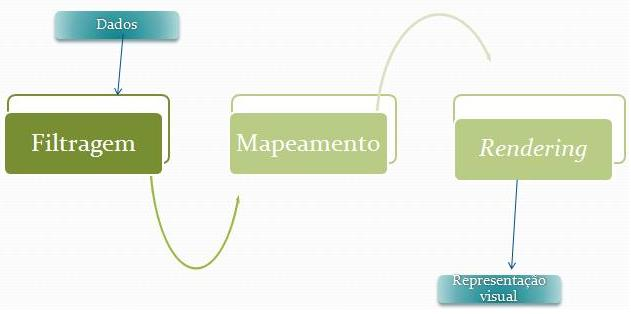
\includegraphics[height=6cm,width=10cm]{imagens-proposta/vis-class.jpg}
\caption{Modelo cl�ssico de visualiza��o \cite{HABER}.}
\label{fig:rep1}
\end{figure}
\begin{figure}[h]
\centering
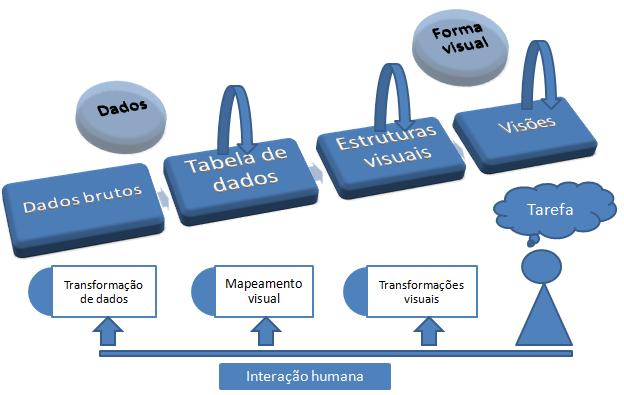
\includegraphics[height=6cm,width=11cm]{imagens-proposta/ref-vis.jpg}
\caption{Modelo de refer�ncia de visualiza��o \cite{CAR99}.}
\label{fig:rep2}
\end{figure}
\subsection{Vantagens}
\label{secao:vantagens-visualizacao}
Dentre as vantagens que podem ser associadas ao uso de VISINFO podem ser citadas as seguintes \cite{NASCIMENTO}: 
\begin{itemize}
\item Uma grande quantidade de informa��es pode ser condensada em apenas uma �nica e simples imagem que representa essa informa��o de forma a ser facilmente entend�vel;
\item O processo de visualiza��o trabalha com o sentido humano da vis�o, que � o mais capaz de perceber informa��es por unidade de tempo. O sentido da vis�o � paralelo e r�pido, sendo poss�vel prestar aten��o em determinado objeto sem perder de vista (obviamente, com menos detalhes) o que est� acontecendo ao redor;
\item O sentido humano da vis�o � treinado para reconhecer padr�es, sendo poss�vel identificar e lidar com diversos novos problemas do cotidiano com a utiliza��o de padr�es j� vistos e que envolvam o processamento visual de informa��es. A constata��o de padr�es ou caracter�sticas visuais presentes em imagens contribui de forma significativa para o processo de compreens�o, mais do que a simples observa��o dos dados em sua forma bruta.
\end{itemize}
\par A constru��o de uma visualiza��o que possibilite a observa��o desses padr�es pode ser obtida organizando os dados segundo algum crit�rio definido e apresentando-os de modo visual. Isto se torna vantajoso, pois une uma grande quantidade de informa��o relevante que estava dispersa em uma ou v�rias formas visuais, facilitando a an�lise desses dados e consequente uso da maior quantidade de informa��o poss�vel.
\subsection{Aplica��es}
\label{secao:aplicacoes-visualizacao}
As t�cnicas de VISINFO t�m sido utilizadas em diversas �reas tais como: monitoramento de bolsas de valores e estudo de mercados; consultas a bancos de dados atrav�s de t�cnicas de \textit{data mining}, envolvendo �reas como jogos, tend�ncias de consumo de produtos e sistemas de informa��es geogr�ficos e engenharia de \textit{software}, atrav�s da utiliza��o de visualiza��es que auxiliem o programador a analisar e entender o funcionamento de um programa, em um n�vel maior de abstra��o quando comparado a uma simples an�lise do c�digo fonte. 
\par As t�cnicas de VISINFO t�m sido usadas tamb�m na �rea de redes de computadores com a finalidade de realizar an�lises da grande quantidade de dados gerados, aplicando filtros sobre esses dados a fim de perceber padr�es que essas redes apresentam, e apresentando v�rias informa��es simultaneamente em uma �nica imagem.
\subsection{T�cnicas}
\label{secao:tecnicas-visualizacao} 
As t�cnicas de VISINFO procuram representar graficamente dados de um determinado dom�nio de aplica��o de forma que, a partir das rela��es espaciais exibidas, o ser humano interprete e compreenda as informa��es apresentadas e, finalmente, deduza novos conhecimentos. Elas t�m o potencial de auxiliar na an�lise visual e explora��o de grandes conjuntos de dados, atrav�s do emprego de mecanismos que buscam tanto representar visualmente os dados, quanto permitir ao usu�rio a intera��o com estas representa��es. 
\par Em uma VISINFO, os dados s�o abstratos e n�o h� necessariamente uma representa��o geom�trica inerente aos mesmos. Uma imagem � gerada com base nos relacionamentos e informa��es que podem ser inferidos acerca dos dados.
O processo de se gerar uma visualiza��o, basicamente, consiste em mapear os atributos dos dados abstratos em atributos visuais de uma imagem.
Os dados abstratos a serem visualizados podem ser classificados nas seguintes categorias principais \cite{CAR99}:
\begin{itemize}
\item Nominal --- conjunto de elementos distintos, sem uma rela��o de ordem entre eles. Exemplo: mel�o, ma��, melancia, morango;
\item Ordinal --- conjunto de elementos distintos, mas com uma rela��o de ordem entre os mesmos. Exemplo: primeiro, segundo, terceiro, ..., ou segunda, ter�a, quarta, ... ; 
\item Quantitativo --- faixa de valores num�ricos. Essa categoria pode ser dividida em intervalos (com valores discretos) e raz�o (representando uma faixa cont�nua de valores).
\end{itemize}
\par Para o desenvolvimento de sistemas que utilizem t�cnicas de VISINFO deve-se considerar a melhor forma de se mapear informa��es para uma representa��o gr�fica que facilite a sua interpreta��o pelos usu�rios. Deve-se, tamb�m, fornecer meios para limitar ou filtrar a quantidade de informa��o a ser interpretada, mas mantendo o usu�rio ciente do espa�o total de informa��es.
\par � necess�rio, tamb�m, possibilitar formas de manipula��o do conjunto de dados, tanto geom�trica (rota��es e \textit{zoom} na representa��o gr�fica, por exemplo) como analiticamente (redu��o ou expans�o do conjunto de dados exibido de acordo com algum crit�rio determinado pelo usu�rio).
\par De acordo com Card, Mackinlay e Shneiderman \cite{CAR99}, as estruturas dimensionais de representa��o s�o as seguintes: as estruturas unidimensionais, que s�o tipicamente empregadas para a apresenta��o de documentos de texto ou de linhas do tempo, podendo
ser combinadas com um segundo ou terceiro eixo para mostrar compara��o entre valores; as estruturas visuais bidimensionais, como gr�ficos de linhas, barras, pizza e mapas, que s�o mais apropriadas para apresentar dados estat�sticos, descrever fun��es matem�ticas ou visualizar informa��es geogr�ficas; e para dados com \textit{n} dimens�es (\textit{n} maior que 3), quando t�cnicas mais elaboradas s�o necess�rias, tais como, \textit{Multidimensional Scalling}, Coordenadas Paralelas, \textit{treemap}, dispers�o e \textit{Glyphs}.
\par Para ilustrar, a seguir s�o apresentadas brevemente tr�s t�cnicas de VISINFO \cite{prisma}: 
\begin{enumerate}
\item \textit{Treemap} --- t�cnica baseada no preenchimento de espa�os. Os itens s�o ordenados por um valor de atributo que � representado por um ret�ngulo de �rea proporcional ao valor deste atributo. � uma t�cnica ideal para representar dados hier�rquicos e fazer correla��es entre dados e grupos de dados. 
A Figura \ref{fig:tree}, retirada de RDI \cite{prisma}, mostra uma imagem gerada com a utiliza��o da t�cnica de \textit{treemap}.
\begin{figure}[htbp]
\centering
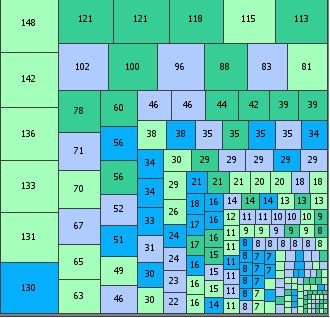
\includegraphics{imagens-relatorio/treemap.jpg}
\caption{Imagem gerada com a utiliza��o da t�cnica de \textit{treemap}, retirada de RDI \cite{prisma}.}
\label{fig:tree}
\end{figure}
\item Dispers�o --- t�cnica baseada na ideia de gr�fico X-Y, ou seja, os eixos s�o configur�veis por atributo. Cada ponto ou coordenada representa um conjunto de valores de atributos. � uma t�cnica ideal para identifica��o de grupos de dados por afinidade de caracter�sticas.
A Figura \ref{fig:dis}, retirada de RDI \cite{prisma}, mostra uma imagem gerada com a utiliza��o da t�cnica de dispers�o.
\begin{figure}[htbp]
\centering
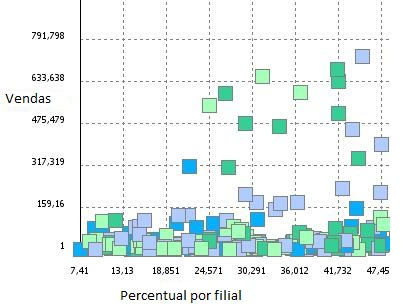
\includegraphics{imagens-relatorio/dispersao.jpg}
\caption{Imagem gerada utilizando a t�cnica de dispers�o, retirada de RDI \cite{prisma}.}
\label{fig:dis}
\end{figure}
\item Coordenadas paralelas --- t�cnica proposta por Inselberg \cite{ins}, mapeia um espa�o \textit{n}-dimensional em uma estrutura bidimensional que usa \textit{n} eixos paralelos verticais equidistantes, denominados coordenadas. Os eixos verticais representam as dimens�es ou atributos dos dados e uma linha representando cada item de dado conecta os eixos nos seus respectivos valores, permitindo a observa��o de padr�es e tend�ncias nos dados \cite{silva}.
A Figura \ref{fig:coo}, retirada de RDI \cite{prisma}, mostra um gr�fico utilizando coordenadas paralelas.
\begin{figure}[htbp]
\centering
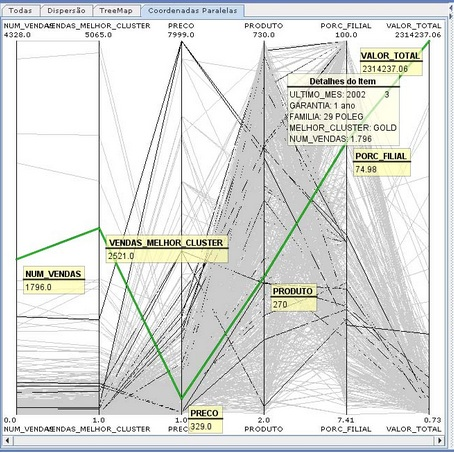
\includegraphics{imagens-tc2/revisao/coordenadasparalelas.jpg}
\caption{Exemplo de gr�fico com coordenadas paralelas, retirado de RDI \cite{prisma}.}
\label{fig:coo}
\end{figure}
\end{enumerate}
\section{Ger�ncia de Redes de Computadores}
\label{secao:gerencia}
\subsection{Introdu��o}
\label{secao:definicao-gerencia}
A �rea de GRC foi inicialmente impulsionada pela necessidade de monitora��o e controle do universo de dispositivos que comp�em as redes de comunica��o. O aumento do grau de complexidade das redes e do seu tamanho exige o emprego de um sistema de gerenciamento que proporcione qualidade de servi�o, pr�-atividade, integra��o com processos de servi�os e de neg�cios. O cont�nuo crescimento em n�mero e diversidade dos componentes de redes de computadores tem tornado a atividade de gerenciamento cada vez mais complexa, e o uso dos servi�os das redes � afetado pela disponibilidade e efici�ncia do gerenciamento feito nas redes de computadores \cite{BRISA}.
\par Atualmente, as redes de computadores e os seus recursos associados t�m se tornado fundamentais e de tal import�ncia para uma organiza��o, que elas ``n�o podem falhar'', sob o risco da organiza��o parar se a rede n�o estiver funcional. Isto significa que o n�vel de falhas e de degrada��o de desempenho considerados aceit�veis est� cada vez mais diminuindo, sendo o n�vel desejado igual ou muito pr�ximo a zero, dependendo da import�ncia da rede para a institui��o \cite{BRISA}.
\par Para resolver os problemas associados da GRC a ISO (\textit{International Organization for Standardization})\abbrev{ISO} {\emph{International Organization for Standardization}} prop�s tr�s modelos para o gerenciamento de redes \cite{BRISA}:
\begin{enumerate}
\item Modelo Organizacional --- estabelece a hierarquia entre sistemas de GRC em um dom�nio de ger�ncia, dividindo o ambiente a ser gerenciado em v�rios dom�nios.
\item Modelo Informacional --- define os objetos de ger�ncia, as rela��es e as opera��es sobre esses objetos. Uma MIB (\textit{Management Information Base})\abbrev{MIB} {\emph{Management Information Base}} � necess�ria para armazenar os objetos gerenciados. 
\item Modelo Funcional --- descreve as funcionalidades de ger�ncia: Gerenciamento de Falhas, Gerenciamento de Configura��o, Gerenciamento de Contabiliza��o, Gerenciamento de Desempenho e Gerenciamento de Seguran�a.
\end{enumerate}
\par Uma forma simples de caracterizar as fun��es de gerenciamento � atrav�s das funcionalidades que envolvem o modelo FCAPS, sigla formada a partir das iniciais de cada �rea de gerenciamento em ingl�s (\textit{Fault, Configuration, Accounting, Performance} e \textit{Security}). Este modelo serve de base para os demais por definir as �reas funcionais da GRC \cite{BRISA}. 
\par O Gerenciamento de Falhas � o respons�vel pelo desenvolvimento de aplica��es que identifiquem as falhas e informem a um gerente a ocorr�ncia dessas, para que decis�es e atitudes sejam tomadas para resolver o problema ocorrido. Com as informa��es sobre falhas ocorridas, a qualidade de servi�o acertada com um usu�rio tende a ser mantida, uma vez que o setor respons�vel pela opera��o e/ou manuten��o da rede antecipa-se aos usu�rios na solu��o de problemas de rede \cite{slides}.
\par O Gerenciamento de Configura��o � a �rea respons�vel pela an�lise, estudo e gerenciamento da topologia e do fluxo de dados da rede atrav�s de ferramentas gr�ficas. 
\par O Gerenciamento de Contabiliza��o � importante para a identifica��o e registro de custos e do volume de recursos utilizados pelos usu�rios de uma rede. 
\par O Gerenciamento de Desempenho � importante n�o para garantir apenas a qualidade de servi�o acordada com os usu�rios, mas tamb�m para assegurar que seja atingida com os menores custos poss�veis. Pode-se por meio do Gerenciamento de Desempenho, adequar os meios de comunica��o utilizados pelos usu�rios �s suas reais necessidades, auxiliando o setor respons�vel pela administra��o da rede, e se antecipado aos usu�rios na manuten��o dos n�veis de desempenho dos servi�os oferecidos, como, por exemplo, o tempo de resposta.
\par O Gerenciamento de Seguran�a � o respons�vel pela monitora��o e controle dos mecanismos de seguran�a de uma rede. Estes mecanismos envolvem desde os mecanismos de controle de acesso aos sistemas computacionais at� o controle de informa��es sigilosas que trafegam na rede. Exemplos destes mecanismos incluem desde prote��o de senhas, com uso de criptografia at� a obrigatoriedade de troca de senha periodicamente. 
\par A Figura \ref{fig:fcaps} apresenta uma forma de integra��o entre as 5 �reas funcionais de GRC \cite{WIKI-pt}. Se as �reas de Seguran�a, de Contabiliza��o, de Falhas e de Configura��o funcionarem de forma adequada, a �rea de Desempenho ser� beneficiada, pois o desempenho de uma rede � diretamente influenciado por problemas ocasionados em uma ou mais das quatro �reas mencionadas.
\begin{figure}[htbp]
\centering
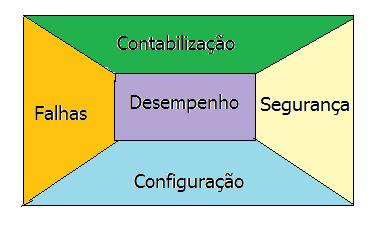
\includegraphics{imagens-proposta/fcaps.jpg}
\caption{Integra��o entre as �reas funcionais de Ger�ncia de Redes \cite{WIKI-pt}.}
\label{fig:fcaps}
\end{figure}
\subsection{Arquitetura de Gerenciamento}
\label{secao:arquitetura-informacao}
Os componentes essenciais de uma arquitetura de gerenciamento de redes s�o \cite{BRISA}:
\begin{itemize}
\item Descri��o da Estrutura de Gerenciamento --- relacionada com as informa��es que podem ser efetuadas sobre os objetos gerenciados (SMI - \textit{Structure Management Information}\abbrev{SMI} {\emph{Structure Management Information}}).
\item Defini��o da Base de Informa��o de Gerenciamento --- lista inicial dos objetos gerenciados (MIB).
\item Protocolos e servi�os --- utiliza��o de protocolos e servi�os de gerenciamento sobre os protocolos de transporte TCP (\textit{Transmission Control Protocol})\abbrev{TCP} {\emph{Transmission Control Protocol}} ou UDP (\textit{User Datagram Protocol})\abbrev{UDP} {\emph{User Datagram Protocol}}.
\end{itemize}
\par Uma SMI define como s�o identificadas e descritas as informa��es gerenciadas. A MIB � especificada utilizando a SMI e cont�m os objetos a serem gerenciados.
\par Um exemplo de SMI � a SMI Internet, projetada para ser uma estrutura de informa��o dependente de um protocolo, por exemplo, o protocolo SNMP (\textit{Simple Network Management Protocol})\abbrev{SNMP} {\emph{Simple Network Management Protocol}} \cite{BRISA}.
\subsection{MIB}
\label{secao:mib}
Um objeto gerenciado � a vis�o abstrata de um recurso real do sistema. Assim, todos os recursos da rede que devem ser gerenciados s�o modelados, e as estruturas de dados resultantes s�o os objetos gerenciados. Os objetos gerenciados podem ter permiss�es para serem lidos ou alterados, sendo que cada leitura representar� o estado real do recurso e, cada altera��o tamb�m ser� refletida no pr�prio recurso \cite{artola}.
\par Dessa forma, a MIB � o conjunto dos objetos gerenciados, que procura abranger todas as informa��es necess�rias para a ger�ncia da rede, possibilitando assim, a automatiza��o de grande parte das tarefas de ger�ncia.
\par O RFC (\textit{Request for Comments})\abbrev{RFC} {\emph{Request for Comments}} 1066 \cite{rfc} apresentou a primeira vers�o da MIB para uso com o protocolo TCP/IP, a MIB-1. Este padr�o explicou e definiu a base de informa��o necess�ria para monitorar e controlar redes baseadas no protocolo TCP/IP. O RFC 1066 foi aceito pela IAB (\textit{Internet Activities Board})\abbrev{IAB} {\emph{Internet Activities Board}} como padr�o no RFC 1156. O RFC 1158 prop�s uma segunda MIB, a MIB-2, para uso com o protocolo TCP/IP, sendo aceita e formalizada como padr�o no RFC 1213. A MIB-2 expandiu a base de informa��es definidas na MIB-1.
\par A MIB-2 usa uma arquitetura de �rvore, definida na ISO ASN.1 (\textit{Abstract Syntax Notation.1})\abbrev{ASN.1} {\emph{Abstract Syntax Notation.1}}, para organizar todas as suas informa��es. Cada parte da informa��o da �rvore � um n� rotulado que cont�m um OID (\textit{Object IDentifier})\abbrev{OID} {\emph{Object IDentifier}}, ou seja, uma sequ�ncia de n�meros separados por pontos e uma pequena descri��o textual \cite{artola}. Um exemplo de objeto est� descrito a seguir:
\begin{verbatim}
directory(1)
identificador de objetos: 1.3.6.1.1
descri��o textual: {internet 1}
\end{verbatim}
\par Um n� rotulado pode ter sub�rvores contendo outros n�s rotulados. Caso n�o tenha sub�rvores, ele � um n� folha e ser� um objeto que cont�m um valor. Na Figura \ref{fig:mib2} � apresentada a �rvore que representa a MIB-2.
\begin{figure}[height=4cm,width=4cm]
\centering
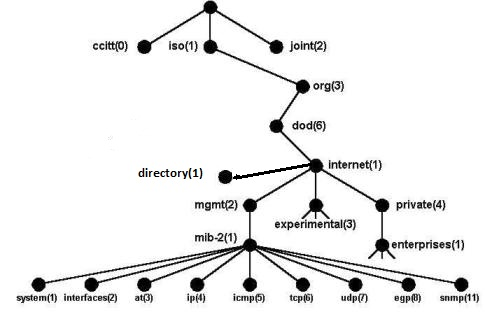
\includegraphics{imagens-relatorio/mib2-this.jpg}
\caption{A MIB-2.}
\label{fig:mib2}
\end{figure}
\par O n� raiz da �rvore MIB-2 n�o tem nome ou n�mero, mas tem tr�s sub�rvores:
\begin{enumerate}
\item \textit{ccitt(0)}, administrada pelo CCITT (Comit� Consultivo Internacional de Telegrafia e Telefonia)\abbrev{CCITT} {Comit� Consultivo Internacional de Telegrafia e Telefonia}.
\item \textit{iso(1)}, administrada pela ISO.
\item \textit{joint-iso-ccitt(2)}, administrada pela ISO juntamente com o CCITT.
\end{enumerate}
Sob o n� \textit{iso(1)}, est�o outras sub�rvores, como � o caso da sub�rvore \textit{org(3)}, definida pela ISO para conter outras organiza��es. Uma das organiza��es que est� sob a sub�rvore \textit{org(3)} � o DOD (\textit{Departament of Defense of USA})\abbrev{DOD} {\emph{Departament of Defense of USA}}, no n� \textit{dod(6)}. A \textit{Internet(1)} est� sob o \textit{dod(6)}, e possui quatro sub�rvores:
\begin{enumerate}
\item \textit{directory(1)}: cont�m informa��es sobre o servi�o de diret�rios OSI (\textit{Open Systems Interconnection})\abbrev{OSI} {\emph{Open Systems Interconnection}}.
\item \textit{mgmt(2)}: cont�m informa��es de gerenciamento, � sob esta sub�rvore que est� o n� da \textit{mib-2}, com o identificador de objeto 1.3.6.1.2.1 ou \verb!{ mgmt 1 }!.
\item \textit{experimental(3)}: cont�m os objetos que ainda est�o sendo pesquisados pela IAB.
\item \textit{private(4)}: cont�m objetos definidos por outras organiza��es.
\end{enumerate}
\par Abaixo da sub�rvore \textit{mib-2} est�o os objetos usados para obter informa��es espec�ficas dos dispositivos da rede. Esses objetos s�o divididos em 11 grupos, que s�o apresentados na Tabela \ref{tab3} e detalhados a seguir, com as respectivas �reas FCAPS que cada grupo abrange \cite{artola}. Na Tabela \ref{tab:exemplos} s�o apresentados alguns exemplos de objetos pertencentes a cada um dos grupos.
\begin{table}[h]
\begin{center}
\caption{�reas FCAPS dos grupos da sub�rvore \textit{mib-2}.}
\begin{tabular}{|l||c|c|c|c|c|c|}
\hline
\multicolumn{7}{|c|}{MIB-2} \\ \hline \hline
\multicolumn{1}{|c||}{Grupos} & Informa��o & F & C & A & P & S \\ \hline
\textit{system}(1) & Sistema de opera��o & $\bullet$ & $\bullet$ & & & \\
\textit{interfaces}(2) & Interface da rede & $\bullet$ & $\bullet$ & $\bullet$ &$\bullet$ & \\ 
\textit{address translation}(3) & Mapeamento de endere�os IP & & & & & \\
\textit{ip}(4) & Protocolo IP & $\bullet$ & $\bullet$ & $\bullet$ & $\bullet$ & \\
\textit{icmp}(5) & Protocolo ICMP & & & & $\bullet$ & \\
\textit{tcp}(6) & Protocolo TCP & & $\bullet$ &$\bullet$ & $\bullet$ & $\bullet$\\
\textit{udp}(7) & Protocolo UDP & & $\bullet$ & $\bullet$ & $\bullet$ & \\
\textit{egp}(8) & Protocolo EGP & $\bullet$ & $\bullet$ & $\bullet$ &$\bullet$ & \\
\textit{cmot}(9) & Protocolo CMOT & & & & & \\
\textit{transmission}(10) & Meios de transmiss�o & & & & & \\
\textit{snmp}(11) & Protocolo SNMP & $\bullet$ &$\bullet$ & $\bullet$ &$\bullet$ & $\bullet$ \\
\hline
\end{tabular}
\label{tab3}
\end{center}
\end{table}
%\begin{enumerate}
%\item \textit{system(1)}: O grupo \textit{system} cont�m informa��es b�sicas sobre o sistema gerenciado. Muitos dos objetos desse grupo s�o usados no gerenciamento de configura��o e gerenciamento de falhas. 
%\item \textit{interfaces(2)}: O grupo \textit{interfaces} oferece dados sobre cada interface de um dispositivo gerenci�vel da rede. Essas informa��es s�o �teis para o gerenciamento de falhas, de configura��o, de desempenho e de contabiliza��o.
%\item \textit{at(3)}: O grupo \textit{address translation} n�o constitui mais um grupo separado. Seus objetos foram incorporados aos grupos de outros protocolos.
%\item \textit{ip(4)}: O IP � um protocolo de rede que utiliza um modo de servi�o sem conex�o para entregar datagramas. O grupo IP prov� informa��es sobre o protocolo IP no dispositivo. Estas informa��es s�o subdivididas em quatro grupos: erros e tipos de pacotes IP, endere�os IP, tabela de roteamento e mapeamento de endere�os IP (substituindo o grupo \textit{address translation}). Os objetos do grupo \textit{ip} podem ser aplicados ao gerenciamento de falhas, de configura��o, de desempenho e de contabiliza��o.
%\item \textit{icmp(5)}: O ICMP � um protocolo que carrega mensagens de erro e controle para dispositivos IP. O grupo \textit{icmp} cont�m objetos que fornecem informa��es sobre o protocolo ICMP na dispositivo gerenciado. Todos os seus objetos s�o aplicados ao gerenciamento de desempenho. 
%\item \textit{tcp(6)}: O TCP � um protocolo de transporte que prov� conex�es confi�veis entre aplica��es. Muitas implementa��es do TCP incluem recursos adicionais para lidar com controle de fluxo, congestionamento da rede, e a retransmiss�o de segmentos perdidos. O grupo \textit{tcp} � utilizado no gerenciamento de configura��o, de desempenho, de contabiliza��o e de seguran�a.
%\item \textit{udp(7)}: O UDP � um protocolo de transporte que, ao contr�rio do TCP, n�o garante seguran�a e nem estabelece conex�es. Ao inv�s disso, ele usa um fluxo de datagramas para transportar as informa��es. O grupo \textit{udp} possui um n�mero limitado de objetos e � usado no gerenciamento de desempenho, de contabiliza��o e de configura��o.
%\item \textit{egp(8)}: O EGP (\textit{Exterior Gateway Protocol})\abbrev{EGP} {\emph{Exterior Gateway Protocol}} � um protocolo que informa a um dispositivo de rede IP como alcan�ar outras redes IP. Ele n�o informa a rota completa para a outra rede, mas ela permite que um dispositivo saiba em que dire��o que a rede existe. Redes IP podem ser agrupadas em �reas l�gicas chamadas sistemas aut�nomos. Um sistema aut�nomo geralmente � uma rede e suas sub-redes associadas ou uma cole��o de redes e sub-redes sob uma mesma administra��o. Dois dispositivos de rede em dois sistemas aut�nomos distintos podem compartilhar informa��es de alcance via EGP. Os objetos do grupo EGP podem ser aplicados ao gerenciamento de falhas, de configura��o, de desempenho e de contabiliza��o.
%\item \textit{cmot(9)}: O grupo \textit{cmot} existe somente por raz�es hist�ricas. Para efetuar a transi��o do SNMP para outro protocolo de gerenciamento, o CMIP (\textit{Common Management Information Protocol})\abbrev{CMIP} {\emph{Common Management Information Protocol}}, foi criado o protocolo CMOP (\textit{CMIP Over TCP/IP})\abbrev{CMOP} {\emph{CMIP Over TCP/IP}} para auxiliar nesta tarefa. No entanto, embora a defini��o para o CMOT exista, nenhum trabalho significativo tem sido feito em cima deste protocolo h� algum tempo, e logo n�o h� nenhum objeto neste grupo. O principal problema do CMIP se tornar um padr�o na ind�stria � o fato dele ser orientado � conex�o, ao contr�rio do SNMP que envia dados sem solicitar explicitamente uma conex�o.
%\item \textit{transmission(10)}: O grupo \textit{transmission} prov� informa��es sobre o meio espec�fico que forma a base das interfaces no sistema. Quando os padr�es Internet para gerenciar v�rios tipos de meios forem definidos, este grupo ser� o prefixo para estas informa��es.
%\item \textit{snmp(11)}: O grupo \textit{snmp} informa desde erros referentes a mensagens SNMP at� objetos que informam a porcentagem que uma entidade est� utilizando para manipular o SNMP. Os erros que ocorrem neste protocolo n�o constituem erros de rede em si, mas podem informar que a entidade n�o est� manipulando os pacotes apropriadamente.
%Os objetos do grupo \textit{snmp} podem ser aplicados em todas as cinco �reas de gerenciamento. Aplica��es de gerenciamento de falhas observando problemas SNMP podem achar �til conhecer o n�mero de erros e sua frequ�ncia, enquanto aplica��es de gerenciamento de desempenho podem calcular a taxa de pacotes entrando e deixando a entidade. J� aplica��es de gerenciamento de contabiliza��o podem usar os objetos SNMP para encontrar o n�mero de pacotes enviados ou recebidos pela entidade. E por fim, alguns objetos do grupo \textit{snmp} podem ajudar no gerenciamento de configura��o e seguran�a. 
%\end{enumerate}
\begin{table}[htb]
\begin{center}
\caption{Exemplos de objetos da \textit{mib-2} e seus respectivos grupos.}
\begin{tabular}{|c|c|c|}
\hline
Grupo & \multicolumn{2}{|c|}{Objeto --- Informa��o (descri��o) utilizada no gerenciamento} \\
\hline
1 & \textit{sysDescr} & Descri��o do sistema \\ 
& \textit{sysLocation} & Localiza��o f�sica do sistema \\
& \textit{sysUpTime} & Quanto tempo o sistema est� operacional \\
\hline 
2 & \textit{ifDescr} & Nome da interface \\
& \textit{ifSpeed} & Largura de banda da interface \\ 
\hline 
% 3 & & \\
% \hline
4 & \textit{ipInReceives} & Taxa de datagramas de recebidos \\ 
& \textit{ipInAddrErrors} & Taxa de erros de endere�o de entrada \\
& \textit{ipForwDatagrams} & Taxa de datagramas repassados \\
\hline 
5 & \textit{icmpInMsgs} & Taxa de recebimento de mensagens \\
& \textit{icmpInErrors} & Taxa de erros de entrada \\
\hline
6 & \textit{tcpInErrs} & N�mero de pacotes recebidos com erro\\
& \textit{tcpInSegs} & Taxa de segmentos TCP recebidos\\
& \textit{tcpOutSegs} & Taxa de segmentos TCP enviados \\
\hline 
7 & \textit{udpInDatagrams} & Taxa de datagramas recebidos \\
& \textit{udpInErrors} & Taxa de datagramas UDP recebidos com erro\\
\hline 
8 & \textit{egpInMsgs} & Taxa de mensagens recebidas \\
& \textit{egpInErrors} & Taxa de mensagens recebidas com erro \\
& \textit{egpOutMsgs} & Taxa de mensagens enviadas \\
\hline 
% 9 & & \\
% \hline 
% 10 & & \\
% \hline
11 & \textit{snmpInPkts} & Taxa de pacotes SNMP recebidos \\
& \textit{snmpOutPkts} & Taxa de pacotes SNMP enviados \\
\hline
\end{tabular}
\label{tab:exemplos}
\end{center}
\end{table}
\par Cada objeto contido nos grupos apresentados na Tabela \ref{tab:exemplos} � descrito no RFC 1213. A descri��o dos objetos � dividida em cinco partes: o nome do objeto, a sintaxe abstrata do objeto, a descri��o textual do significado do objeto (nome completo, vers�o, etc.), o tipo de acesso permitido ao objeto (\textit{read-only}, \textit{read-write}, \textit{write-only} ou n�o acess�vel) e o estado do objeto (obrigat�rio, opcional ou obsoleto). 
O exemplo a seguir apresenta a descri��o do objeto \verb!sysDescr { Internet 1 }!.
\begin{verbatim}
 OBJECT
  sysDescr {Internet 1}
  Syntax: DisplayString(SIZE(0..255))
  Description: "A textual description of the entity. 
  This value should include the full name and version identification of the 
  system's hardware type, software operating-system and networking software.
  It is mandatory that this only contain printable ASCII characters."
  Access: read-only
  Status: mandatory
\end{verbatim}
\subsection{Protocolo SNMP}
\label{secao:snmp}
\par Com a crescente necessidade de Gerenciamento de Redes de Computadores, fez-se necess�rio que padr�es para o desenvolvimento de protocolos fossem estabelecidos. O SNMP � um protocolo de ger�ncia de redes TCP/IP (\textit{Transmission Control Protocol/ Internet Protocol})\abbrev{TCP/IP} {\emph{Transmission Control Protocol/Internet Protocol}}, da camada de aplica��o que facilita o interc�mbio de informa��es entre os dispositivos de rede, como placas e \textit{switches}, possibilitando aos administradores de rede encontrar e resolver eventuais problemas na rede e prover informa��es sobre os equipamentos gerenciados \cite{WIKI-pt}. O SNMP � usado para administrar o desempenho de uma rede, encontrar e resolver problemas de rede e planejar o crescimento da mesma. � utilizado em servidores, roteadores, \textit{firewalls}, \textit{switches}, \textit{hubs}, impressoras, \textit{modens}, equipamentos remotos, multiplexadores, etc.
\par Os componentes chaves de uma rede gerenciada pelo protocolo SNMP s�o os seguintes:
\begin{itemize}
\item Esta��o de Gerenciamento;
\item Agente de Gerenciamento;
\item MIB;
\item Protocolo de Gerenciamento de Redes.
\end{itemize}
\par A esta��o de gerenciamento serve como interface para o gerente humano em um sistema de gerenciamento de rede.
O agente de gerenciamento responde �s solicita��es de informa��es e de a��es da esta��o de gerenciamento e deve tamb�m prover assincronamente informa��es importantes que n�o foram solicitadas por esta esta��o.
Os recursos a serem gerenciados s�o representados como objetos, e a cole��o de objetos � referenciada como uma MIB.
A forma de comunica��o entre a esta��o de gerenciamento e o agente � definida por um protocolo de gerenciamento de rede, por exemplo, o SNMP.
\par No escopo deste protocolo, definem-se os elementos de rede classificados como cliente (ou gerente) respons�vel pela monitora��o e controle dos \textit{gateways} e \textit{hosts}, que correspondem aos servidores (ou agentes).
\par O protocolo SNMP � baseado no paradigma conhecido como ``busca-armazenamento'' (\textit{fetch-store}), isto �, todas as opera��es previstas por este protocolo s�o derivadas de opera��es b�sicas de busca e armazenamento. As mensagens desse protocolo n�o possuem campos fixos e s�o especificadas na nota��o ASN.1. O SNMP sugere que a l�gica do servidor de objetos de um equipamento seja colocada no agente e este execute opera��es elementares, como estabelecer e obter valores das vari�veis. O programa que analisa, manipula, combina ou aplica algum algoritmo sobre os dados deve residir no gerente \cite{BRISA}. 
\par Geralmente, o SNMP � executado sobre o UDP e o IP (\textit{Internet Protocol})\abbrev{IP} {\emph{Internet Protocol}}, e n�o sobre o TCP, mas � importante ressaltar que o gerenciamento de redes n�o � semelhante �s outras aplica��es de rede. Quando tudo falha, o gerenciamento da rede deve continuar funcionando e deve ser capaz de usar a parte mais simples do protocolo de rede (um protocolo de datagrama n�o-confirmado) para chegar ao equipamento gerenciado. Os projetistas do SNMP optaram pelo uso de protocolos n�o orientados a conex�o por medo, em caso de falha, de ser imposs�vel estabelecer uma conex�o \cite{BRISA}, al�m de considerarem o desempenho do protocolo UDP \textit{versus} o protocolo TCP.
\par O gerenciamento de rede atrav�s do SNMP permite o acompanhamento simples e f�cil do estado, em tempo real, da rede, podendo ser usado para gerenciar diferentes tipos de sistemas. Cada m�quina gerenciada pelo SNMP deve possuir um agente e uma base de informa��es MIB, que � um conjunto de vari�veis que representam informa��es referentes ao seu estado atual, estas informa��es ficam dispon�veis ao gerente atrav�s de consulta e podem ser alteradas por ele.
\par No protocolo SNMPv1 existem as opera��es: \textit{set}, \textit{get}, \textit{get-next} e \textit{trap}. J� o protocolo SNMPv2 inseriu melhorias nas opera��es de \textit{trap} e inseriu duas novas opera��es: \textit{get-bulk} e \textit{inform}.
\begin{itemize}
\item A opera��o \textit{set} � utilizada para alterar o valor da inst�ncia de um objeto em um cliente;
\item A opera��o \textit{get} � utilizada para ler o valor de uma inst�ncia de um objeto; o gerente solicita que o agente obtenha e retorne o valor;
\item A opera��o de \textit{get-next} � utilizada para ler o valor da pr�xima inst�ncia de um objeto; o gerente fornece o
nome de uma vari�vel e o cliente obt�m o valor e o nome da pr�xima inst�ncia de um objeto; tamb�m �
utilizado para obter valores e nomes de objetos de uma tabela de tamanho desconhecido;
\item A opera��o \textit{trap} � utilizada para comunicar um evento; o agente comunica ao gerente o acontecimento de um evento, previamente determinado. No SNMPv2, a opera��o de \textit{trap} possui a mesma fun��o que no SNMPv1, por�m, usa diferentes formatos de mensagens e foi implementada com o objetivo de substituir a primeira vers�o. 
\item A opera��o \textit{get-bulk} � usada para a busca de uma grande quantidade de dados, como informa��es presentes em uma tabela. Esta opera��o � uma otimiza��o em rela��o � opera��o de \textit{get}. 
\item A opera��o \textit{inform} no SNMPv2 permite a comunica��o entre os gerentes em uma rede.
\end{itemize}
\subsection{Gerenciamento de Desempenho}
\label{secao:gerenciamento-desempenho}
\par O Gerenciamento de Desempenho consiste em um conjunto de fun��es respons�veis pela manuten��o e exame dos registros que cont�m o hist�rico dos estados de um sistema. Seu objetivo � analisar as tend�ncias do uso dos componentes e definir um planejamento atrav�s do dimensionamento dos recursos que devem ser alocados para o sistema. Isto � feito atrav�s da monitora��o das atividades da rede e do controle dos recursos atrav�s de ajustes e trocas. Assim, s�o atendidos os requisitos dos usu�rios deste sistema, satisfazendo as suas demandas, ou seja, garantindo que n�o ocorram insufici�ncias de recursos quando sua utiliza��o se aproximar da capacidade total do sistema.
\par As fun��es de Gerenciamento de Desempenho podem ser divididas em dois grupos \cite{BRISA}:
\begin{itemize}
\item Medidas de Tr�fego: estas fun��es possibilitam ao usu�rio definir e controlar a entrega de relat�rios de medidas de tr�fego.
\item Monitora��o de Desempenho: s�o informa��es que permitem ao usu�rio obter, avaliar e relatar par�metros de desempenho da rede. Tais informa��es podem ser utilizadas como apoio ao diagn�stico de falhas, ao planejamento da rede e � qualidade do servi�o.
\end{itemize}
\par Para atingir os objetivos de desempenho desej�veis, deve-se monitorar a taxa de utiliza��o dos recursos, a taxa em que estes recursos s�o pedidos e a taxa em que os pedidos a um recurso s�o rejeitados. Para cada tipo de monitora��o, � definido um valor m�ximo aceit�vel (\textit{threshold}), um valor de alerta e um valor em que se remove a situa��o de alerta.
\par Na Ger�ncia de Desempenho tem-se a possibilidade de avaliar o comportamento dos recursos em um ambiente de gerenciamento para verificar se este comportamento � eficiente, ou seja, preocupa-se com o desempenho corrente da rede, atrav�s de par�metros estat�sticos como atrasos, vaz�o, disponibilidade e o n�mero de retransmiss�es realizadas. 
\par Algumas das quest�es relativas ao gerenciamento do desempenho s�o \cite{especial}:
\begin{itemize}
\item Qual � o n�vel de capacidade de utiliza��o?
\item O \textit{throughput} foi reduzido para n�veis aceit�veis?
\item O tr�fego � excessivo?
\item Existem gargalos?
\item O tempo de resposta est� aumentando?
\end{itemize}
Para tratar estas quest�es, o gerente de uma rede de computadores deve focar em um conjunto inicial de recursos a serem monitorados, a fim de estabelecer n�veis de desempenho. Isto inclui associar m�tricas e valores apropriados aos recursos de rede que possam fornecer indicadores de diferentes n�veis de desempenho. Muitos recursos devem ser monitorados para se obter informa��es sobre o n�vel de opera��o da rede. Colecionando e analisando estas informa��es, o gerente da rede pode ficar mais e mais capacitado no reconhecimento de situa��es indicativas de degrada��o de desempenho.
Estat�sticas de desempenho podem ajudar no planejamento, administra��o e manuten��o de grandes redes. Estas informa��es podem ser utilizadas para reconhecer situa��es de gargalo antes que elas causem problemas para o usu�rio final. A��es corretivas podem ser executadas, tais como, trocar tabelas de roteamento para balancear ou redistribuir a carga de tr�fego durante hor�rios de pico, ou ainda, a longo prazo, indicar a necessidade de expans�o de linhas para uma determinada �rea \cite{especial}.
%--------------------------------------------------------------------------------------------
\chapter{Trabalhos Relacionados}
\label{capitulo:relacionados}
Dentre os trabalhos relacionados com o Desview (apresentado no Cap�tulo \ref{capitulo:trab}) s�o apresentadas neste cap�tulo quatro ferramentas utilizadas largamente na ind�stria e tr�s trabalhos acad�micos:
\begin{itemize}
\item Cacti;
\item Nagios;
\item MRTG;
\item OpenNMS;
\item \textit{Management Traffic Analyzer};
\item Prisma;
\item Visualiza��o e An�lise de Dados de Monitoramento de Sistemas usando Multi-resolu��o.
\end{itemize}
\section{Cacti}
\label{secao:cacti}
O Cacti \cite{CACTI} � uma ferramenta industrial que coleta informa��es sobre o estado de uma rede de computadores e as exibe atrav�s de gr�ficos. Foi desenvolvido para ser flex�vel, de modo a se adaptar facilmente a diversas necessidades, bem como ser robusto e f�cil de usar. Dentre as funcionalidades do Cacti est�o a monitora��o do estado de elementos de rede e programas, bem como largura de banda utilizada e uso de CPU (\textit{Central Processing Unit})\abbrev{CPU} {\emph{Central Processing Unit}}.
\par O Cacti utiliza a ferramenta \textit{RRDTool} \cite{rrdtool}, ou seja, uma ferramenta para criar bases de dados respons�veis por armazenar os dados recolhidos e por gerar os gr�ficos. O RRD (\textit{Round Robin Database})\abbrev{RRD} {\emph{Round Robin Database}} foi desenvolvido para armazenar s�ries de dados num�ricos sobre o estado de uma rede de computadores, por�m pode ser empregado no armazenamento de qualquer outra s�rie de dados como temperatura, uso de CPU, etc. As informa��es s�o repassadas para a ferramenta atrav�s de \textit{scripts} ou outros programas escolhidos pelo usu�rio que devem se encarregar de obter os dados. Pode-se utilizar tamb�m o protocolo SNMP para consultar informa��es em elementos de redes e/ou programas que suportam tal protocolo.
\par O Cacti � uma solu��o gr�fica de rede projetada para aproveitar as funcionalidades do \textit{RRDTool} como armazenamento de dados e gr�ficos. O Cacti proporciona modelos gr�ficos avan�ados, v�rios m�todos de aquisi��o de dados, gerenciamento de usu�rios e de recursos. Todas essas funcionalidades s�o acessadas atrav�s de uma interface gr�fica \textit{web} podendo ser utilizado desde redes pequenas at� redes complexas, com centenas de dispositivos.
\par Um exemplo de gr�fico gerado pelo Cacti pode ser observado na Figura \ref{fig:cacti}. Nessa figura � apresentada a quantidade de mem�ria utilizada, em \textit{kilobytes}, por um elemento de rede, em um intervalo de tempo (no caso 5 em 5 minutos, padr�o no Cacti).
\begin{figure}[h] %Outros parametros: t=top, b=bottom
\centering
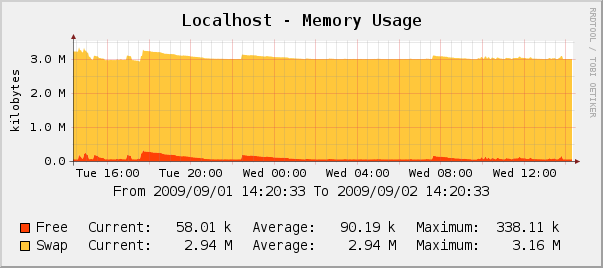
\includegraphics[width=10cm, height=10cm]{imagens-proposta/cacti.png}
\caption{Exemplo de gr�fico gerado pelo Cacti \cite{CACTI}.}
\label{fig:cacti}
\end{figure}
\section{MRTG}
\label{secao:mrtg}
O MRTG (\textit{Multi Router Traffic Grapher})\abbrev{MRTG}{\emph{Multi Router Traffic Grapher}} \cite{mrtg} � uma ferramenta de monitora��o que gera p�ginas \abbrev{HTML}{\emph{HyperText Markup Language}} com gr�ficos de dados coletados a partir de SNMP ou \textit{scripts} externos. � conhecido principalmente pelo seu uso na monitora��o de tr�fego de rede, utilizando dados solicitados via comandos SNMP a um determinado \textit{host}.
\par Foi desenvolvido por Tobias Oetiker e Dave Rand em Perl utilizando um m�dulo em C para gerar os gr�ficos. O MRTG � uma ferramenta comumente utilizada para monitorar tr�fego em interfaces de rede, mas pode monitorar muitas outras vari�veis, tais como utiliza��o de disco r�gido, temperatura de \textit{hardware} e uso de processador, podendo gerar alertas a partir de \textit{thresholds}, facilitando, assim, o gerenciamento da rede. 
O princ�pio de funcionamento do MRTG � relativamente simples: o programa � executado periodicamente para consultar as informa��es do banco de dados (MIB) dos equipamentos de acordo com um arquivo de configura��o. O resultado desta consulta � usado para construir gr�ficos que s�o armazenadas em uma p�gina do diret�rio \textit{web}. Feito isto, o MRTG permite analisar graficamente atrav�s de um navegador, a tend�ncia do tr�fego de entrada e sa�da de um \textit{host}. 
\par O MRTG tem como prop�sito apresentar na forma de gr�ficos 2D medidas estat�sticas dos dados de dispositivos de rede (\textit{switches}, roteadores e \textit{hubs}), utilizando o protocolo de captura de dados de rede SNMP.
\par S�o algumas caracter�sticas do MRTG \cite{mrtg}:
\begin{itemize}
\item Possuir op��es que permitem personalizar a forma como ela opera;
\item Coleta dados a cada 5 minutos por padr�o, mas este tempo pode ser alterado;
\item Cria uma p�gina HTML com 4 gr�ficos (di�rio, semanal, mensal e anual). Se algum deles n�o for necess�rio pode ser eliminado;
\item Pode avisar caso o valor do gr�fico atinja um valor pr�-estabelecido. Por exemplo: se determinado servidor atinge 95\% do espa�o do disco, o MRTG pode mandar um \textit{email} para o administrador informando o ocorrido;
\item Possui uma ferramenta para gerar os arquivos de configura��o: o CFGMAKER e outra ferramenta para gerar uma p�gina de �ndice para os casos em que muitos itens s�o monitorados: o INDEXMAKER.
\end{itemize}
\par Exemplos de gr�ficos di�rio, semanal, mensal e anual gerados pelo MRTG podem ser observados na Figura \ref{fig:mrtg}, retirados de Switch \cite{switch}. Nos gr�ficos s�o mostrados a m�dia de \textit{bits} recebidos e enviados em gr�ficos com os valores di�rios, semanais, mensais e anuais coletados da rede.
\begin{figure}
\centering
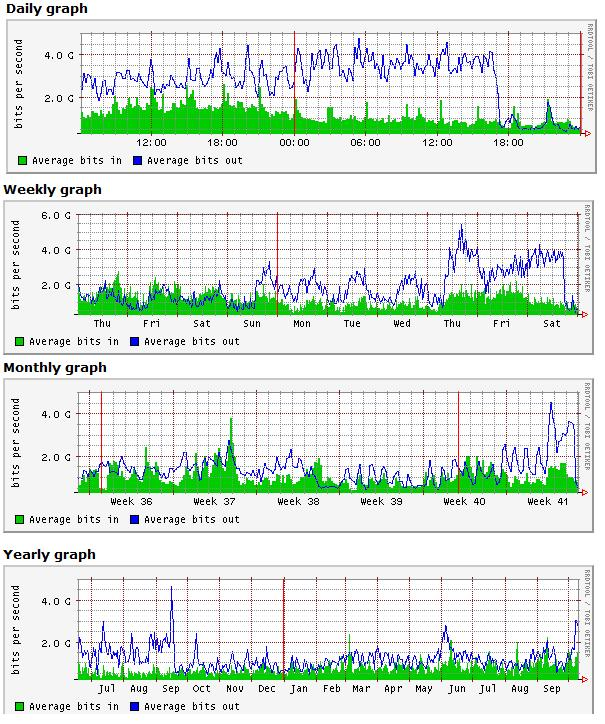
\includegraphics{imagens-relatorio/mrtg.jpg}
\caption{Imagens geradas pelo MRTG, retiradas de Switch \cite{switch}.}
\label{fig:mrtg}
\end{figure}
\section{Nagios}
\label{secao:nagios}
O Nagios \cite{NAGIOS} � uma aplica��o, tamb�m industrial, de monitora��o de rede de c�digo aberto e licenciado pelo sistema GPL (\textit{GNU General Public License})\abbrev{GPL}{\emph{GNU General Public License}}. Ele pode monitorar tanto \textit{hosts} quanto servi�os, gerando alertas quando ocorrerem problemas e tamb�m quando os problemas forem resolvidos.
O Nagios foi originalmente desenvolvido com o nome de Netsaint, foi escrito e � atualmente mantido por Ethan Galstad, juntamente com um conjunto de desenvolvedores que ativamente disponibilizam \textit{plugins} oficiais e n�o-oficiais.
\par As principais funcionalidades que o Nagios oferece s�o:
\begin{itemize}
\item Monitora��o de diversos servi�os de rede (SNMP, ICMP\abbrev{ICMP}{\emph{Internet Control Message Protocol}}, TCP, HTTP\abbrev{HTTP}{\emph{Hypertext Transfer Protocol}} e outros);
\item Monitora��o de recursos de computadores ou equipamentos de rede (carga do processador, uso de disco e \textit{logs} do sistema);
\item Capacidade de notificar quando um servi�o ou equipamento apresenta problemas e quando o problema � resolvido (via \textit{email}, mensagem de texto no celular ou qualquer outro meio definido pelo usu�rio atrav�s de um \textit{plugin});
\item Interface \textit{web} para visualiza��o do atual \textit{status} da rede, notifica��es, hist�rico de problemas, arquivos de \textit{log}, etc.
\end{itemize}
\par Um exemplo de gr�fico gerado pela ferramenta Nagios pode ser observado na Figura \ref{fig:nagios}. Nessa figura � apresentado o uso de CPU, com valores m�ximos, m�dia e �ltimo valor lido pelos diversos processos de um elemento de rede em um intervalo de tempo.
\begin{figure}[h]
\centering
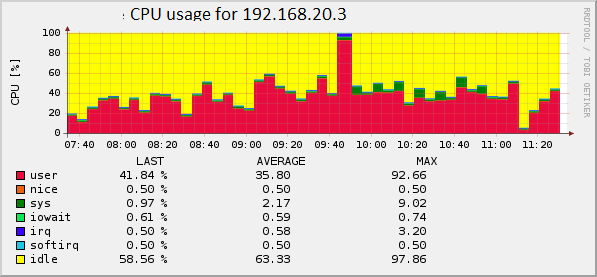
\includegraphics[width=10cm]{imagens-tc2/revisao/nagios.png}
\caption{Exemplo de gr�fico gerado pelo Nagios \cite{NAGIOS}.}
\label{fig:nagios}
\end{figure}
\section{OpenNMS}
\label{secao:trabalho-opensource-1}
O OpenNMS \cite{opennms} � um projeto \textit{open-source} desenvolvido em Java, dedicado � cria��o de uma plataforma de ger�ncia de rede voltada principalmente para a camada de aplica��o. Nele � poss�vel visualizar as informa��es do tipo \cite{opennms-pdf}:
\begin{itemize}
\item estado dos servi�os e interfaces de rede;
\item disponibilidade geral dos servi�os;
\item eventos gerados;
\item gr�ficos de desempenho;
\item informa��es sobre equipamentos.
\end{itemize}
\par Dentre as funcionalidades do OpenNMS pode-se citar a descoberta de recursos e servi�os, o \textit{polling} configur�vel dos equipamentos, calend�rio de manuten��o onde se pode definir per�odos em que haver� manuten��es que possam afetar a disponibilidade de servi�o, coleta de dados atrav�s de leituras SNMP, execu��o de comandos quando determinados \textit{thresholds} forem violados, gr�ficos estat�sticos de utiliza��o, de falhas de \textit{buffer}, de erros \textit{in/out}, de descartes, dentre outros \cite{opennms-pdf}.
\par Na Figura \ref{fig:opennms}, tem-se um exemplo de gr�fico que a ferramenta OpenNMS gera, onde � poss�vel verificar 4 vari�veis da MIB-2 sendo tendo seus valores monitorados e plotados em um gr�fico.
\begin{figure}[!h]
\centering
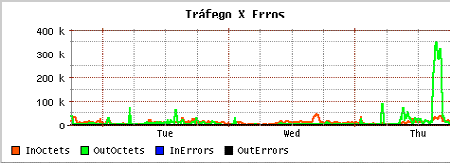
\includegraphics[width=8cm, height=5cm]{imagens-tc2/opennms.png}
\caption{Exemplo de gr�fico gerado pelo OpenNMS.}
\label{fig:opennms}
\end{figure}
\section{Ferramenta \textit{Management Traffic Analyzer}}
\label{secao:trabalho-academico-1}
O trabalho realizado por Salvador e Granville \cite{SALVADOR} tem por objetivo apresentar atrav�s de t�cnicas de VISINFO, os resultados de an�lises obtidos com medi��es do tr�fego SNMP, utilizando a ferramenta \textit{Management Traffic Analyzer}, desenvolvida para automatizar este processo. A ferramenta foi implementada sobre SNMPDUMP (programa que analisa tr�fego SNMP), invocando as fun��es de SNMP quando necess�rio. As an�lises s�o realizadas por \textit{scripts} escritos em Perl, e o resultado dessas an�lises s�o armazenadas em um banco de dados MySQL. A seguir, t�cnicas de visualiza��o implementadas como aplicativos usando \textit{Macromedia Flash ActionScript} permitem a visualiza��o gr�fica das informa��es armazenadas. De acordo com Salvador e Granville \cite{SALVADOR}, o uso de t�cnicas de visualiza��es foi importante porque elas permitiram explorar e obter vis�es do tr�fego SNMP, facilitando a descoberta de padr�es de tr�fego, anomalias e disparidades. No trabalho foram apresentadas visualiza��es baseadas em t�cnicas visuais, como a apresentada na Figura \ref{fig:acad1}, na qual � demonstrado atrav�s de um histograma o n�mero de mensagens SNMP que trafegaram pela rede em cada hora durante determinado dia.
\par A ferramenta apresentada prop�e um conjunto limitado de t�cnicas para visualizar informa��es espec�ficas relacionadas com o SNMP atrav�s de medi��es de tr�fego. Estas visualiza��es s�o capazes de gerar gr�ficos, por�m seria necess�rio aumentar o conjunto de t�cnicas de visualiza��o dispon�veis na ferramenta, a fim de melhorar o potencial de vis�o sobre o tr�fego SNMP, j� que a enorme quantidade de informa��es geradas por v�rios dispositivos e sistemas que comp�em as redes modernas demanda cada vez mais esfor�os para o entendimento dessas informa��es.
\begin{figure}[h]
\centering
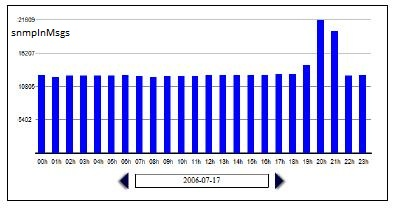
\includegraphics[width=10cm]{imagens-proposta/mta.jpg}
\caption{Gr�fico gerado pela ferramenta \textit{Management Traffic Analyzer} \cite{SALVADOR}.}
\label{fig:acad1}
\end{figure}
\section{Ferramenta Prisma}
\label{secao:trabalho-academico-2}
A ferramenta Prisma, desenvolvida por Kauer \cite{KAUER}, � uma aplica��o que utiliza VISINFO atrav�s de t�cnicas de m�ltiplas coordenadas para explorar conjuntos de dados de uma rede de computadores. Tr�s t�cnicas conhecidas de visualiza��o s�o usadas: \textit{treemap}, dispers�o e coordenadas paralelas \cite{HABER}. A ferramenta utiliza um conjunto de dados proveniente de \textit{logs} de elementos de rede contendo informa��es como endere�o IP, porta e protocolo utilizado, quantidade de \textit{bytes} enviados e recebidos e estado da opera��o (sucesso, redirecionamento, falha, etc.).
\par O Prisma foi desenvolvido para ajudar na an�lise de situa��es em que grandes volumes de dados s�o envolvidos. A ferramenta � composta por v�rias formas de visualiza��o gr�fica que permitem aos usu�rios a an�lise dos dados e das rela��es entre eles.
\par A Figura \ref{fig:acad2} apresenta um exemplo de gr�fico gerado pela ferramenta que, de acordo com Kauer \cite{KAUER}, possui as seguintes caracter�sticas:
\begin{itemize}
\item Extens�vel, port�til e de f�cil manuten��o uma vez que foi desenvolvida em Java utilizando \textit{design patterns};
\item A interface gr�fica � automaticamente personalizada de acordo com o tipo e o intervalo de valores de dados de cada conjunto;
\item Possui filtros que possibilitam ao usu�rio analisar informa��es que ele deseja em determinado momento;
\item Oferece relat�rios de barras, linhas e outras formas gr�ficas que s�o gerados automaticamente pela ferramenta.
\end{itemize}
\begin{figure}[h] 
\centering
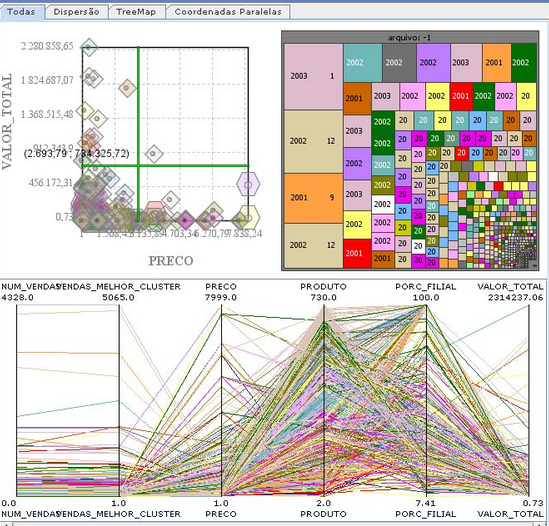
\includegraphics[width=15cm]{imagens-tc2/revisao/prisma.png}
\caption{Gr�fico com as tr�s t�cnicas utilizadas no Prisma (\textit{treemap}, dispers�o e coordenadas paralelas) para o mesmo conjunto de dados de entrada \cite{KAUER}.}
\label{fig:acad2}
\end{figure}
\section{Visualiza��o e An�lise de Dados de Monitoramento de Sistemas usando Multi-resolu��o}
\label{secao:nayak}
O trabalho realizado por Nayak, Neogi e Kothari \cite{nayak} explora a natureza multi-resolu��o do monitoramento de dados 
e representa��es de eventos de dados para a constru��o de uma topologia que preserve vis�es para o monitoramento de informa��es. De acordo com Nayak, Neogi e Kothari \cite{nayak}, o sistema desenvolvido � um \textit{framework} que representa
eventos de dados ocorridos. Eventos s�o normalmente produzidos em certas opera��es de monitoramento de dados, por
exemplo, um evento pode corresponder ao fato de o espa�o livre em um disco estar abaixo de 10\%. Ao inv�s de 
serem observados os pontos m�ximos ocorridos de eventos, o que normalmente ocorre, � desej�vel que seja visualizado
e entendido o comportamento das complexas infraestruturas que comp�em os sistemas atuais. O \textit{framework} proposto
� baseado em arranjos e cada fonte de dados monitorada � organizada de forma hier�rquica para refletir as inter-rela��es
entre as diferentes fontes de dados monitoradas. No trabalho apresentado s�o utilizadas redes neurais \cite{rdn} baseadas em Mapas Auto-Organiz�veis \cite{som} para gerar as visualiza��es a partir dos 
eventos gerados pelos elementos monitorados, assim, os Mapas Auto-Organiz�veis produzem uma topologia preservando o mapeamento em diversas dimens�es.
\par A Figura \ref{fig:som} mostra um exemplo de Mapa Auto-Organiz�vel apresentado no trabalho, no qual se mostra a constru��o de um mapa topol�gico onde os nodos mais pr�ximos respondem de forma semelhante a padr�es de entrada semelhantes a eles, j� a Figura \ref{fig:acad3} apresenta uma representa��o da organiza��o baseada em arranjos, retirada de Nayak \cite{nayak}. Nela � demonstrado o resultado obtido do mapeamento de dados em 6D para 2D no \textit{framework} desenvolvido.
\begin{figure}[h] 
\centering

\includegraphics[width=4cm, height=4cm]{imagens-relatorio/som.jpg}
\caption{Exemplo de um Mapa Auto-Organiz�vel retirado de Germano \cite{som}. O mapa bi-dimensional gerado representa as posi��es dos nodos em rela��o aos nodos vizinhos. O objetivo � que os nodos que forem topologicamente pr�ximos respondam de maneira semelhante a entradas semelhantes.}
\label{fig:som}
\end{figure}
\begin{figure}[h]
\centering
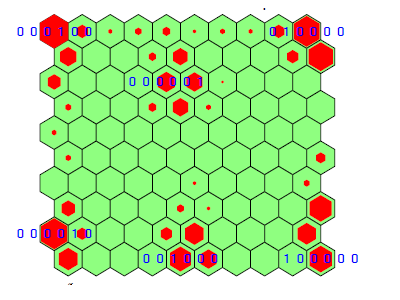
\includegraphics[width=11cm]{imagens-relatorio/mul.png}
\caption{Mapeamento de dados de entrada 6-D em 2-D atrav�s de Mapas Auto-Organiz�veis, onde os dados de entrada correspondem a 6 diferentes vetores com apenas um n�mero `1' em cada vetor. Figura retirada de Nayak \cite{nayak}.}
\label{fig:acad3}
\end{figure}


\chapter{Descri��o do Desview}
\label{capitulo:trab} 
Neste cap�tulo s�o apresentados os objetivos, o ambiente de desenvolvimento utilizado, a modelagem, a interface e as funcionalidades, a implementa��o do prot�tipo e um estudo de caso do trabalho que foi desenvolvido.
\section{Introdu��o}
\label{secao:introducao-trab}
O objetivo deste trabalho � o projeto e o desenvolvimento de um sistema de monitora��o de desempenho de elementos em uma rede de computadores que a partir de dados coletados por monitora��es via protocolo SNMP, utilizando t�cnicas de VISINFO sobre os mesmos, de modo que o usu�rio verifique os estados e dados de vari�veis em equipamentos com base nas visualiza��es que s�o apresentadas. Assim, caso os valores de vari�veis que est�o em monitoramento passem de valores pr�-definidos, as visualiza��es informem de maneira f�cil ao usu�rio que a vari�vel em monitora��o saiu do intervalo do qual � considerado dentro do desempenho considerado normal.
\par S�o requisitos do prot�tipo que foi desenvolvido:
\begin{itemize}
\item Permitir a defini��o de quais par�metros ser�o monitorados;
\item Estabelecer par�metros das medidas de desempenho a serem realizadas;
\item Agendar o monitoramento dessas medidas;
\item Permitir a consulta, a altera��o, a inclus�o e a exclus�o de medidas;
\item Armazenar os resultados obtidos;
\item Apresentar os dados obtidos durante as medi��es atrav�s de diferentes 
representa��es visuais.
\end{itemize}
\section{Ambiente de desenvolvimento}
\label{secao:ambiente}
Para a implementa��o do sistema proposto foi utilizada a linguagem de programa��o Java, a biblioteca OpenGL para a gera��o das representa��es visuais, e a biblioteca SNMP4J para a comunica��o com o protocolo SNMP dos elementos de rede monitorados.
\par A biblioteca OpenGL � composta por um conjunto de fun��es, que fornecem acesso a praticamente todos os recursos do \textit{hardware} de v�deo. 
Internamente, ela age como uma m�quina de estados, que de maneira bem espec�fica diz � placa de v�deo o que deve ser feito. Usando as fun��es da biblioteca, pode-se especificar, ligar ou desligar v�rios aspectos dessa m�quina, tais como a cor atual, a transpar�ncia que ser� usada, os par�metros de ilumina��o, efeitos de neblina, entre outros \cite{manssour}.
\par Para a implementa��o de gr�ficos onde � usada sele��o de objetos em OpenGL foi utilizada a biblioteca \textit{Graphic Engine API} \cite{Jouvieje}, que possui m�todos que facilitam a sele��o e manipula��o de formas gr�ficas em OpenGL. Escolheu-se utilizar esta API devido a problemas encontrados durante o desenvolvimento de gr�ficos que necessitavam de sele��o de objetos, e esta mostrou-se ser uma biblioteca simples com maior facilidade de implementa��o da funcionalidade desejada.
\par A linguagem Java foi utilizada para o desenvolvimento por ser uma linguagem livre utilizada em larga escala na ind�stria, possuir uma grande variedade de \textit{frameworks} que facilitam a programa��o al�m de ser port�vel e orientada a objeto. Foi utilizada a biblioteca OpenGL para Java (JOGL \cite{JOGL}), devido ao fato de ela ter implementa��o para \textit{hardware} de v�deo, permitindo desenhar, criar superf�cies e imagens 3D em 
tempo real. J� a biblioteca SNMP4J \cite{SNMP4J} � uma implementa��o \textit{open source} das primitivas SNMP para a linguagem Java, fornecendo v�rias funcionalidades para facilitar a comunica��o entre uma aplica��o e um agente SNMP de determinado elemento de rede.
\par Tamb�m foi utilizado o PostgreSQL \cite{Postgres} como banco de dados para o armazenamento das informa��es, por ser de c�digo aberto, de alta performance, est�vel e que possui in�meros recursos como integridade transacional, controle de concorr�ncia e suporte para chaves estrangeiras e gatilhos. Al�m disso, possui capacidade de lidar com grandes volumes de dados, o que � normalmente gerado pelas redes de computadores atuais. Os gr�ficos 2D s�o implementados utilizando as bibliotecas JFreeChart \cite{jfreechart} e ChartDirector \cite{chartdirector}.
\par Como ferramentas de desenvolvimento foram utilizados os seguintes \textit{softwares}: plataforma de programa��o \textit{NetBeans} \cite{netbeans}, ferramentas de modelagem \textit{UML}\abbrev{UML} {\emph{Unified Modeling Language}} \textit{Jude Community} \cite{jude} e de banco de dados \textit{Power*Architect} \cite{db}. 
\par Foram utilizados, tamb�m, a biblioteca Swingx \cite{swingx}, a biblioteca Quartz \cite{quartz} e o \textit{framework} Hibernate \cite{hibernate} no desenvolvimento das interfaces gr�ficas, escalonamento e persist�ncia de dados, respectivamente. A Swingx � uma extens�o da biblioteca Swing do Java que cont�m componentes aprimorados com in�meras funcionalidades no desenvolvimento de aplica��es, contendo componentes como 
calend�rios, pain�is ``dobr�veis'', componentes que informam que o sistema est� processando alguma requisi��o, dentre outros. A biblioteca Quartz � um escalonador de tarefas, no qual se pode indicar a data e hora exata na qual se deseja executar um trabalho. O Hibernate � um \textit{framework} para o mapeamento objeto-relacional escrito na linguagem Java que facilita o mapeamento dos atributos entre uma base tradicional de dados relacionais e o modelo objeto de uma aplica��o. O objetivo do Hibernate � diminuir a complexidade entre os programas Java, baseado no modelo orientado a objeto, que precisam trabalhar com um banco de dados do modelo relacional (presente na maioria dos sistemas de bancos de dados), principalmente no desenvolvimento de consultas e atualiza��es dos dados \cite{hibernate}.
\section{Modelagem do prot�tipo}
\label{secao:modelagem}
Nesta se��o s�o apresentados os diagramas UML que foram modelados para a implementa��o do prot�tipo, utilizando a ferramenta \textit{Jude Community} \cite{jude}. A Figura \ref{casos-de-uso} apresenta os casos de uso, ou seja, uma an�lise dos requisitos levantados para o sistema, que s�o os seguintes:
\begin{itemize}
\item Criar, excluir e atualizar tarefas e equipamentos;
\item Inserir, excluir e atualizar vari�veis de tarefas;
\item Parar e iniciar tarefas;
\item Exportar dados estat�sticos;
\item Consultar dados persistidos em banco;
\item Estabelecer e atualizar par�metros de desempenho para as vari�veis 
monitoradas;
\item Gerar gr�ficos e visualiza��es sobre os dados coletados.
\end{itemize}
\begin{figure}
\centering
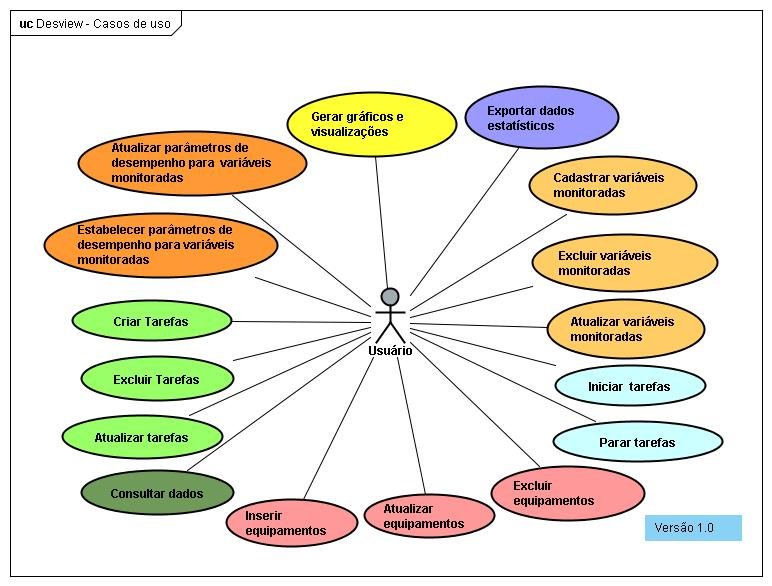
\includegraphics[width=17cm, height=20cm]{imagens-tc2/usecase.jpg}
\caption{Casos de uso do sistema.}
\label{casos-de-uso}
\end{figure}
\par Os diagramas de atividades que detalham os casos de uso apresentados encontram-se no Anexo A e modelo conceitual de classes do prot�tipo encontra-se no Anexo B. 
\par O sistema foi implementado utilizando o padr�o de arquitetura de \textit{software} \textit{MVC} (\textit{model-view-controller})\abbrev{MVC} {\emph{Model-view-controller}}, onde os dados (\textit{model}) s�o separados da interface (\textit{view}) do sistema. Assim, altera��es feitas na interface n�o interferem na 
manipula��o dos dados, assim como estes tamb�m podem ser reorganizados sem alterar a interface. O MVC resolve este problema atrav�s da separa��o das tarefas de acesso aos dados e l�gica de neg�cio, l�gica de apresenta��o e de intera��o com o usu�rio, introduzindo um componente entre os dois: o \textit{controller}. Outros padr�es de projetos utilizados na implementa��o foram: o padr�o \textit{facade} para o acesso SNMP e o padr�o \textit{DAO} (\textit{Data Access Object})\abbrev{DAO} {\emph{Data Access Object}} para acesso ao banco de dados.
\par O prot�tipo possui os seguintes pacotes principais: \textit{model}, \textit{controller}, \textit{util}, \textit{graphics}, \textit{charts} e \textit{view}. Os pacotes s�o apresentados brevemente a seguir e os diagramas de classes destes encontram-se no Anexo B.
\par O pacote \textit{model} cont�m as entidades do sistema, respectivas classes DAO de cada entidade e classes de utilidades usadas nas entidades.
\par S�o caracter�sticas das entidades:
\begin{itemize}
\item \textsl{Equipment}: entidade que representa um equipamento a ser monitorado na rede, possui atributos como endere�o IP, nome, comunidade de escrita e de leitura, \textit{timeout} nas chamadas SNMP, quantidades de \textit{retries} de acesso ao equipamento.
\item \textsl{Variable}: entidade que representa uma vari�vel da MIB, como atributos possui \textit{oid}, nome, \textit{thresholds}, tipo da vari�vel e tipo de acesso.
\item \textsl{Task}: entidade que representa uma tarefa que � executada. Cada tarefa possui vari�veis associadas, um equipamento, data de in�cio, data de fim e frequ�ncia de leitura.
\item \textsl{Reading}: entidade que representa as leituras efetuadas pelas tarefas. Cada leitura cont�m data em que foi realizada, valor lido, tarefa e vari�vel associada.
\item \textsl{Historic}: � uma entidade que representa o hist�rico de leituras j� efetuadas.
\item \textsl{Search}: � uma entidade que guarda todas as pesquisas efetuadas no sistema.
\item \textsl{Users}: � uma entidade que cont�m os usu�rios do sistema. Somente usu�rios cadastrados podem acessar o sistema.
\end{itemize}
\par O pacote \textit{model} cont�m, tamb�m, as classes DAO do sistema e enumera��es utilizadas nas entidades. 
O modelo DAO � um modelo para persistir dados em banco de dados relacional que permite separar regras de neg�cio das regras de acesso a banco de dados. 
As classes de utilidades s�o enumera��es para tipos de dados das entidades, como estado de uma tarefa, tipos de usu�rio, etc.
\par As classes do pacote \textit{controller}, s�o as classes de controle a cada uma das entidades e �s classes DAO. O pacote SNMP cont�m fachadas de acesso aos m�todos SNMP (\textit{get}, \textit{set}, \textit{getNext} e \textit{walk}) e um leitor que l� vari�veis de uma MIB em formato XML.\abbrev{XML} {\emph{Extensible Markup Language}} 
\par O pacote \textit{util} do sistema cont�m as classes de escalonamento de leituras do sistema, de exporta��o de dados e classes de mensagens de erros e de avisos.
\par O pacote \textit{graphics} cont�m as visualiza��es em OpenGL do sistema, s�o apresentadas janelas de escolha dos dados a serem visualizados e a seguir os dados s�o renderizados nas classes \textit{Renderers} de cada pacote; s�o apresentadas visualiza��es em linhas, em espirais e em esferas.
\par O pacote \textit{charts} cont�m os gr�ficos implementados utilizando as ferramentas ChartDirector e JFreeChart. S�o apresentados gr�ficos convencionais de tempo real e gr�ficos polar, de linhas e de barras est�ticos com dados armazenados no banco de dados.
\par E o pacote \textit{view} cont�m as janelas e interfaces gr�ficas do sistema, como inser��o de equipamentos e de tarefas, edi��o de dados, consulta, altera��o de senha, exporta��o de dados coletados de leituras SNMP e demais opera��es do sistema.
\par Na Figura \ref{banco} � apresentado o diagrama do banco de dados relacional gerado na ferramenta \textit{Power*Architect} \cite{db}, mostrando as tabelas e relacionamentos. As tabelas apresentadas ilustram como foram representadas as tabelas do banco de dados atrav�s do mapeamento das entidades (classes) do Hibernate. 
Cada entidade gerou uma tabela do banco de dados, al�m de uma tabela de relacionamento entre as entidades \textit{Task} e \textit{Variable}.
\begin{figure}
\centering
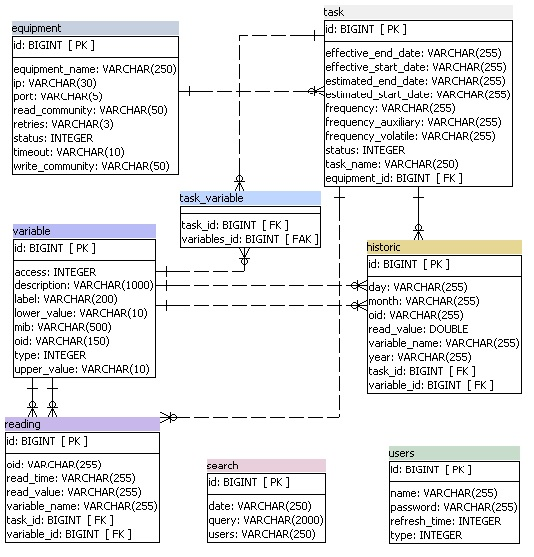
\includegraphics[width=15cm, height=20cm]{imagens-tc2/banco.jpg}
\caption{Modelagem do banco de dados do sistema.}
\label{banco}
\end{figure}
\newpage
\section{Interface e funcionalidades}
\label{secao:interface}
Nesta se��o s�o apresentadas as interfaces gr�ficas e funcionalidades do sistema desenvolvido.
\par A Figura \ref{fig:telaprincipal1} mostra a janela principal do prot�tipo, a qual se tem acesso �s tarefas que est�o sendo monitoradas, criar, editar, parar e iniciar tarefas. Tamb�m se tem acesso as visualiza��es do sistema: visualiza��es OpenGL e gr�ficos convencionais. Na Figura \ref{fig:insercaovariaveisetarefas}, � poss�vel visualizar a tela de inser��o de tarefas e de vari�veis associadas que ser�o lidas pelo escalonador de tarefas. Cada tarefa possui uma data de in�cio, uma data de fim e uma frequ�ncia na qual ser� efetuada a leitura de todas as vari�veis que forem associadas a ela.
\par Outras funcionalidades do prot�tipo s�o: a altera��o e exclus�o de tarefas, de vari�veis e de equipamentos monitorados, a defini��o e altera��o de valores de \textit{thresholds} de cada vari�vel, busca de dados no sistema, inser��o e atualiza��o de usu�rios, al�m da exporta��o de dados de leituras.
\par A Figura \ref{fig:insercaoeq} apresenta a tela de inser��o de equipamentos e a Figura \ref{fig:insercaovariaveisetarefas} mostra a tela de inser��o de tarefas e vari�veis a serem monitoradas.
\par O anexo C apresenta o manual de utiliza��o do prot�tipo e as visualiza��es s�o explicadas em detalhes na se��o \ref{visualizacoes}.
\begin{figure}[!h]
\centering
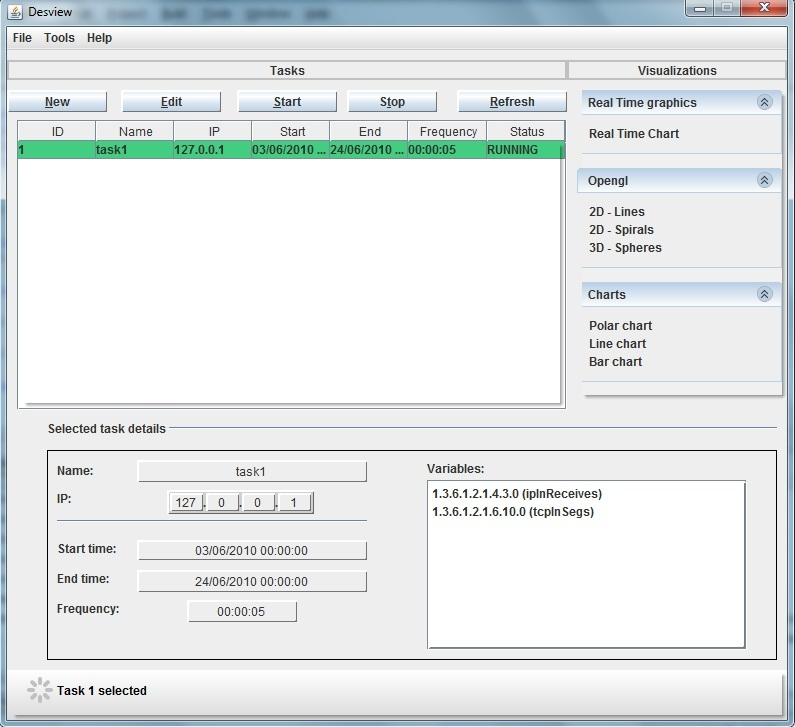
\includegraphics[width=15cm, height=10cm]{imagens-tc2/telas/telaprincipal.jpg}
\caption{Tela principal do prot�tipo.}
\label{fig:telaprincipal1}
\end{figure}
\begin{figure}[!h]
\centering
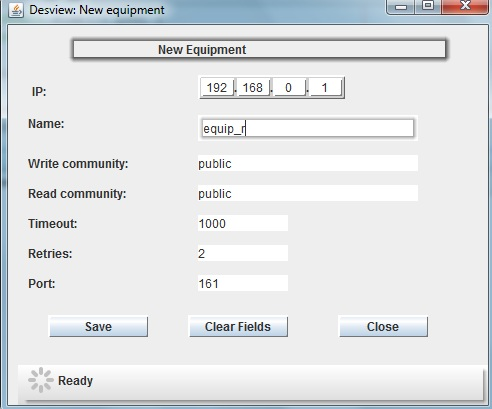
\includegraphics[width=14cm, height=6cm]{imagens-tc2/telas/inserireqtexto.jpg}
\caption{Tela de inser��o de equipamentos.}
\label{fig:insercaoeq}
\end{figure}
\begin{figure}[!h]
\centering
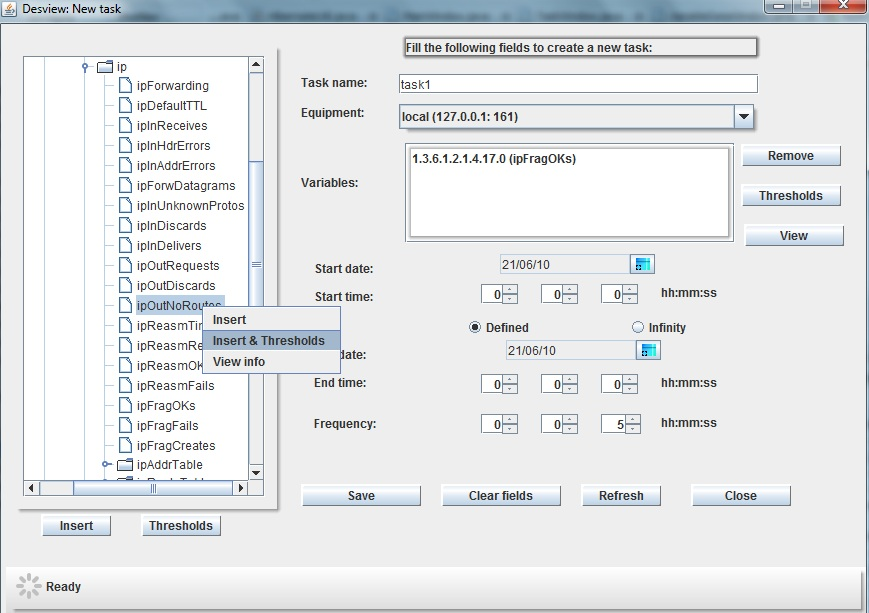
\includegraphics[width=15cm, height=10cm]{imagens-tc2/telas/insercaovariaveisetarefas.jpg}
\caption{Tela de inser��o de tarefas e de vari�veis associadas.}
\label{fig:insercaovariaveisetarefas}
\end{figure}
%----------------------------
\section{Implementa��o}
\label{secao:implementacao}
Nesta se��o � apresentado como foi implementado o prot�tipo, ou seja, 
desde como foi implementada a infraestrutura de banco de dados, as fachadas 
de obten��o de dados SNMP, o escalonador de leituras e as visualiza��es 
implementadas no prot�tipo.
\subsection{Infraestrutura do sistema}
A infraestrutura do sistema implementado � composta dos seguintes mecanismos 
principais:
\begin{itemize}
\item Entidades que correspondem aos objetos armazenados no banco de dados. As classes s�o mapeadas utilizando o Hibernate que controla a inser��o, a atualiza��o e remo��o de dados do banco de dados de cada uma das entidades.
\item Fachada SNMP com os m�todos de acesso �s vari�veis de MIB. O acesso �s vari�veis de uma MIB � feito atrav�s da biblioteca SNMP4J;
\item Gerenciador de tarefas, que realiza o escalonamento, a leitura do valor das vari�veis e posterior inser��o no banco de dados. Como alternativa a este gerenciador de tarefas poderia ter sido utilizado um sistema RRDTool j� implementado, tal como o Cacti, por exemplo, por�m, seria necess�rio um estudo da forma de busca dos dados que s�o armazenados pelo Cacti, o que poderia ser invi�vel para o escopo apresentado. Al�m de utilizar como base de dados o MySQL, tamb�m foi observado que o armazenamento que o Cacti realiza das leituras ocorre em in�meras tabelas com grande n�mero de tabelas de relacionamentos. Por isso, optou-se por implementar uma base de dados mais simples e que se adequasse melhor ao trabalho desenvolvido. Como vantagem do uso de um RRDTool, pode-se citar o controle sobre o ``estouro'' da quantidade de dados e informa��es armazenadas no banco de dados, caracter�stica a qual o sistema implementado n�o possui;
\item Janelas que permitem a inser��o, a altera��o e a exclus�o de equipamentos, de tarefas e de vari�veis, al�m da especifica��o e da atualiza��o dos valores de \textit{thresholds} das vari�veis em monitora��o. Tamb�m, a pesquisa dos dados armazenados, al�m de janelas que filtram dados para a gera��o das visualiza��es;
\item Exporta��o de dados lidos em formato texto e em formato PDF (\textit{Portable Document Format})\abbrev{PDF} {\emph{Portable Document Format}};
\item Sistema de \textit{login}, com altera��es de dados de usu�rios.
\end{itemize}
\subsection{Visualiza��es}
\label{visualizacoes}
Nesta se��o s�o apresentadas as visualiza��es que foram implementadas sobre 
os dados que s�o lidos pelas tarefas do prot�tipo implementado.
\subsubsection{Gr�fico convencionais}
Os gr�ficos convencionais implementados no prot�tipo s�o detalhados a seguir e exemplos s�o apresentados na se��o \ref{secao:estudo-de-caso} - estudo de caso.
\begin{itemize}
\item Gr�fico de barras: exibe as s�ries como conjuntos de barras horizontais. No prot�tipo, os dados que podem ser visualizados s�o a m�dia, o valor m�nimo e o valor m�ximo de cada uma das vari�veis que est�o em monitora��o.
\item Gr�fico polar: exibe uma s�rie como um conjunto de pontos agrupados por categoria em um c�rculo de 360�. � um gr�fico ideal para representar s�ries temporais c�clicas, isto �, s�ries temporais que apresentam em seu desenvolvimento determinada periodicidade. Quanto mais distante o segmento de reta est� do centro, maior � o seu valor. No prot�tipo, os dados que podem ser visualizados atrav�s de gr�fico polar s�o a m�dia dos valores lidos de uma vari�vel durante determinado m�s de um ano.
\item Gr�fico de linhas: um gr�fico de linha � usado para representar grandes quantidades de dados que variam em um per�odo de tempo cont�nuo. No prot�tipo, os dados que podem ser visualizados atrav�s de gr�fico de linhas s�o a m�dia dos valores lidos de uma vari�vel em um ano de monitora��o.
\end{itemize}
%------------
\subsubsection{Gr�fico 2D em linhas}
O gr�fico em OpenGL em linhas tem o seguinte objetivo: dado um conjunto de vari�veis sendo monitoradas por uma tarefa, deseja-se a partir dos \textit{thresholds} inferior e superior de cada uma, verificar atrav�s de linhas coloridas quando uma das vari�veis passa dos intervalos definidos. Assim, a cor da linha informa se o valor atual lido est� abaixo, no intervalo, ou acima dos valores definidos como \textit{thresholds}.
\subsubsection{Gr�fico 2D em espiral}
Durante o desenvolvimento do gr�fico 2D em linhas verificou-se que o desenho de linhas n�o se adequava � grande quantidade de dados que precisam ser plotados, dessa forma, desenvolveu-se o gr�fico OpenGL em espirais que tem o mesmo objetivo do gr�fico 2D em formato de linhas, por�m, o gr�fico em espiral se prop�e a mostrar grande quantidade de dados num espa�o relativamente pequeno. Assim, caso se deseje acompanhar o andamento do gr�fico em linhas � necess�rio acompanhar o desenho movimentando a c�mera ou ent�o redesenhando novamente, o gr�fico em espiral facilita essa atualiza��o, pois ao terminar o espa�o de desenho do gr�fico, apenas inicia-se novamente a espiral.
\subsubsection{Gr�fico 3D em esferas}
O gr�fico 3D de esferas implementado no prot�tipo tem por objetivo, a partir de uma tarefa que se deseja visualizar, plotar um gr�fico 3D informando as m�dias das vari�veis nos meses do ano e o estado da m�dia em rela��o aos \textit{thresholds}, ao clicar em uma das vari�veis em determinado m�s do ano � aberto um novo gr�fico com m�dia dos dias do m�s informando a m�dia em rela��o aos \textit{thresholds}.
%----------------------- estudo de caso -------------------
\section{Estudo de caso}
\label{secao:estudo-de-caso}
O sistema implementado poderia ser utilizado em alguns casos como: controle de taxas de erros (BERT - \textit{bit error rate test}) em equipamentos de redes, que possui um \textit{threshold} superior e se deseja observar se o valor corrente ultrapassa o valor m�ximo desejado durante a realiza��o do teste. Outro caso �til � a monitora��o de sensores de temperaturas, por exemplo. Cada sensor ao conter um agente SNMP embutido, torna-se apto a ser monitorado por um sistema de desempenho que controle a temperatura do mesmo.
\par Assim, nesta se��o s�o apresentados alguns estudos de caso que poderiam ser utilizados como o sistema de gerenciamento de desempenho desenvolvido e que mostrem a utilidade do prot�tipo. S�o utilizadas vari�veis da MIB-2 para ilustrar a sua monitora��o, mas seria interessante usar vari�veis de MIBs propriet�rias, tal como vari�veis de BERT, ou ent�o temperaturas e outros sensores.
\par Dada a seguinte situa��o: utilizando-se um equipamento de rede, deseja-se monitorar o desempenho da vari�vel \textit{icmpInMsgs} da MIB-2. Assim, define-se um \textit{threshold} inferior de 100 e um \textit{threshold} superior de 200 pacotes. Dessa forma ser� utilizado o gr�fico de tempo real para monitorar esta vari�vel, e caso o valor lido ultrapasse o \textit{threshold} estabelecido, uma esp�cie de alarme � mostrado no gr�fico.
Dessa forma, um exemplo do gr�fico obtido monitorando essa vari�vel � apresentado na Figura \ref{fig:graficort}, tornando f�cil verificar que determinada vari�vel passou o \textit{threshold} superior definido, ou ainda est� abaixo do valor definido. Neste trabalho, foi utilizado o desempenho com m�tricas de \textit{thresholds}, mas seria interessante poder monitorar, tamb�m, m�tricas atrav�s de sequ�ncias de c�lculos os quais gerariam taxas e frequ�ncias como m�tricas, por exemplo, taxa de \textit{bytes} que entram em determinada interface de um equipamento de rede, mas por limita��o de tempo e de escopo, optou-se por utilizar m�tricas mais simples com o objetivo de validar o trabalho, mesmo n�o sendo t�o significativas.

\begin{figure}
\centering
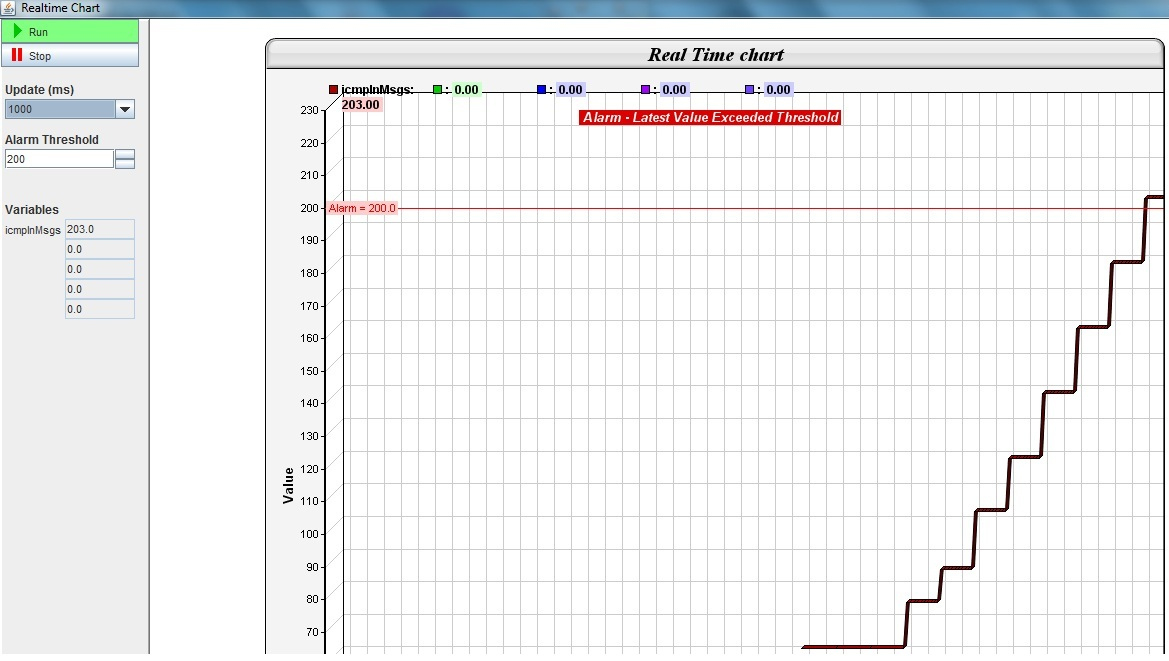
\includegraphics[width=14cm, height=6cm]{imagens-tc2/estudo-caso/graficort.jpg}
\caption{Gr�fico de tempo real obtido, informando que a vari�vel em monitora��o passou do \textit{threshold} informado.}
\label{fig:graficort}
\end{figure}
Utilizando-se a mesma vari�vel apresentada se pode verificar agora qual foi a m�dia de valores lidos durante um m�s de determinado ano. Assim, foi gerado o gr�fico polar da Figura \ref{fig:graficopolar}, contendo a m�dia de cada um dos dias do m�s, no qual � poss�vel verificar em quais dias do m�s o sistema esteve mais sobrecarregado respondendo a requisi��es. Na Figura \ref{fig:graficobarra} tem-se a m�dia, o valor m�ximo e o valor m�nimo dentre as leituras efetuadas. J� a Figura \ref{fig:graficolinha}, apresenta durante os meses de determinado ano, qual foi a m�dia dos valores lidos. Dessa forma, consegue-se por meio dos gr�ficos convencionais apresentados verificar quais foram os pontos em que determinado equipamento foi muito requisitado durante os meses de um ano, e a seguir verificar dentro deste m�s qual foram os dias mais cr�ticos.
\begin{figure}[!h]
\centering
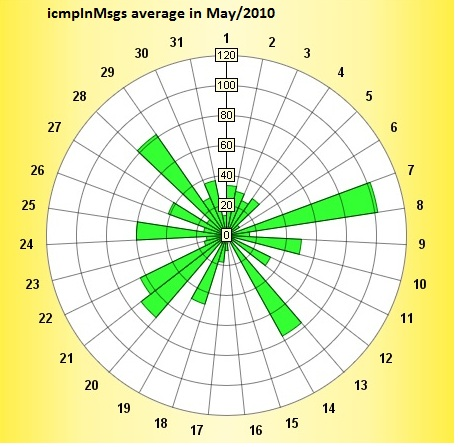
\includegraphics[width=11cm, height=5cm]{imagens-tc2/estudo-caso/polar.jpg}
\caption{Gr�fico polar obtido a partir de leituras efetuadas em uma vari�vel durante um m�s.}
\label{fig:graficopolar}
\end{figure}
\begin{figure}[!h]
\centering
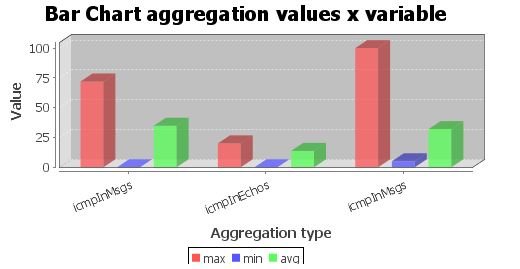
\includegraphics[width=10cm, height=6cm]{imagens-tc2/revisao/bar.png}
\caption{Gr�fico de barras contendo o valor m�nimo, o valor m�ximo e a m�dia dos valores lidos de tr�s vari�veis.}
\label{fig:graficobarra}
\end{figure}
\begin{figure}[!h]
\centering
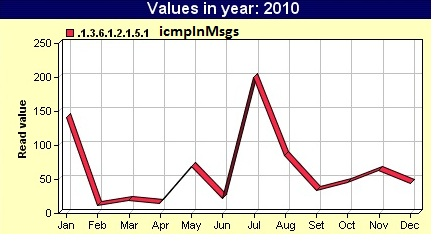
\includegraphics[width=10cm, height=6cm]{imagens-tc2/estudo-caso/linhas.jpg}
\caption{Gr�fico de linhas contendo a m�dia de todos os valores lidos durante os meses de determinado ano.}
\label{fig:graficolinha}
\end{figure}
\par Com os gr�ficos em OpenGL implementados deseja-se verificar como eles podem auxiliar na monitora��o do desempenho da vari�vel em rela��o aos gr�ficos convencionais. Os gr�ficos em OpenGL implementados monitoram vari�veis a partir do seu valor atual com os \textit{thresholds} superior e inferior definidos para cada uma em cada tarefa, ou seja, uma vari�vel pode ter diferentes valores de \textit{thresholds} em diferentes tarefas. As cores presentes nos gr�ficos tem o seguinte significado:
\begin{itemize}
\item Se o valor atual lido for menor que o \textit{threshold} inferior, ent�o desenha o gr�fico com a cor amarela.
\item Se o valor atual lido for maior que o \textit{threshold} superior, ent�o desenha o gr�fico com a cor vermelha.
\item Se o valor atual lido for maior ou igual que o \textit{threshold} inferior e menor ou igual que o \textit{threshold} superior ent�o desenha o gr�fico com a cor verde.
\end{itemize} 
Assim, inicialmente temos o gr�fico 2D de linhas (Figura \ref{fig:2dlinhas}), no qual � poss�vel verificar em um gr�fico que determinada vari�vel saiu de um intervalo de \textit{threshold} e entrou em outro. O mesmo exemplo foi monitorado utilizando o gr�fico em espiral e pode-se observar que a espiral se comportou de forma muito mais satisfat�ria frente a essas mudan�as de estado, principalmente devido ao fato de ela comportar muito mais dados em um espa�o menor (Figura \ref{fig:espiriais}).
\begin{figure}[!h]
\centering

\includegraphics[width=10cm, height=6cm]{imagens-tc2/estudo-caso/2dlinhas1.jpg}
\caption{Gr�fico OpenGL 2D - linhas.}
\label{fig:2dlinhas}
\end{figure}
\begin{figure}[!h]
\centering
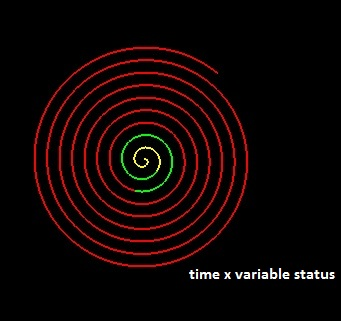
\includegraphics[width=10cm, height=6cm]{imagens-tc2/estudo-caso/espiriais.jpg}
\caption{Gr�fico OpenGL 2D - espirais.}
\label{fig:espiriais}
\end{figure}
\par O objetivo do gr�fico de 3D � a partir de uma tarefa mostrar todas as vari�veis da tarefa em uma linha de tempo contendo os 12 meses do ano. A seguir � analisada a m�dia dos dados coletados em cada um dos meses e a cor da esfera relativa � vari�vel no m�s � colorida de acordo com os crit�rios apresentados anteriormente. Assim, como no exemplo mostrado na Figura \ref{fig:3d1}, na qual se tem um m�s com a m�dia acima dos valores desejados, pode-se clicar na esfera correspondente e passar a verificar o estado da vari�vel nos dias do m�s (Figura \ref{fig:3d2}). Dessa forma, � verificado em que dia a m�dia dos valores foi superior ou inferior aos valores de \textit{thresholds}. Este tipo de gr�fico n�o utiliza dados de leituras em tempo real como os outros gr�ficos OpenGL, ele utiliza a m�dia de todos os valores presentes no banco de dados para as vari�veis que est�o sendo visualizadas. No exemplo apresentado, foram adicionadas mais duas vari�veis de forma a visualizar como ficaria o gr�fico com mais de uma vari�vel.
\begin{figure}[H]
\centering
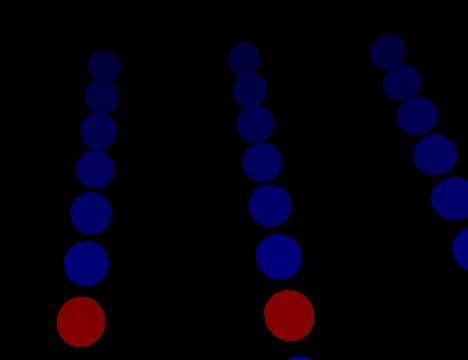
\includegraphics[width=10cm, height=6cm]{imagens-tc2/estudo-caso/3d2.jpg}
\caption{Gr�fico OpenGL 3D - esferas n�vel de var�aveis distribu�das nos meses do ano.}
\label{fig:3d1}
\end{figure}

\begin{figure}[H]
\centering
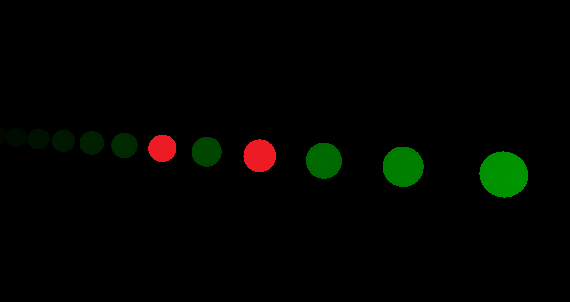
\includegraphics[width=10cm, height=6cm]{imagens-tc2/revisao/3d2.png}
\caption{Gr�fico OpenGL 3D - esferas mostrando os dias do m�s para a vari�vel selecionada.}
\label{fig:3d2}
\end{figure}

\chapter{Conclus�es e trabalhos futuros}
\label{capitulo:conclusoes}
Ao finalizar este Trabalho de Conclus�o pode-se concluir que os conhecimentos adquiridos a partir deste trabalho, foram muito importantes para o desenvolvimento profissional e acad�mico, pois foi poss�vel explorar bibliotecas e tecnologias que n�o haviam sido exploradas em sala de aula. Assim, com a implementa��o deste prot�tipo, iniciou-se um estudo mais aprofundado de uma �rea da Ger�ncia de redes de computadores pouco explorada frente a outras �reas, que s�o consideradas, algumas vezes, mais importantes no gerenciamento de redes, tais como gerenciamento de falhas e de configura��o. \par Com base no problema apresentado, as visualiza��es implementadas t�m por objetivo ilustrar formas de tornar o gerenciamento de desempenho mais f�cil de ser ``gerenciado'', ou seja, sem a necessidade de visualizar grandes quantidades de dados tabulados, mas sim, visualizar os mesmos dados atrav�s de gr�ficos e visualiza��es 2D e 3D que facilitem e auxiliem a verifica��o de que determinada vari�vel est� fora dos padr�es de desempenho considerados aceit�veis.
\par Como trabalhos futuros, pode-se apontar como tarefas, aprofundar o tema em rela��o �s visualiza��es implementadas, al�m de utilizar vari�veis de MIBs que retornem dados relevantes ao gerenciamento de desempenho, presentes na maioria de vezes em MIBs propriet�rias. Al�m disso, pode-se indicar, a implementa��o de novas formas de visualiza��es e o processamento de informa��es vindas da MIB e atrav�s desse processamento obter dados estat�sticos sem utilizar vari�veis espec�ficas de desempenho.
\par Pode-se citar como semelhan�as do prot�tipo implementado com os trabalhos relacionados apresentados: possuir um escalonador de leituras, utilizar visualiza��es atrav�s de gr�ficos convencionais. Como diferencial neste sistema, apresentamos algumas ideias de gr�ficos utilizando a biblioteca OpenGL como apoio para o desenvolvimento de gr�ficos mais elaborados e com possibilidade de mais intera��o, al�m disso, foram exploradas diversas formas geom�tricas proporcionadas pela VISINFO, na busca por melhores formas de representar os dados coletados da rede e que s�o plotados em diversas formas geom�tricas apresentadas. Como desvantagens da prot�tipo desenvolvido, pode-se citar a falta de um agente de descoberta autom�tico, ou seja, toda rede tem que ser adicionada manualmente e tamb�m o fato de n�o ser um sistema Web, ou seja, por ser um aplicativo Java, dificulta o acesso por m�ltiplos usu�rios.


\begin{thebibliography}{100}
%\addcontentsline{toc}{chapter}{Refer�ncias Bibliogr�ficas}

\bibitem{CAR99}
CARD, S.K.; MACKINLAY, J.D.; SHNEIDERMAN, B. \textbf{Readings in Information Visualization - Using Vision to Think}. San Francisco: Morgan Kaufmann Publ., 1999.

\bibitem{ESTIVALET}
ESTIVALET, Luiz Fernando. \textbf{O Uso de �cones na Visualiza��o de Informa��es}. PPGC da UFRGS, 2000.

\bibitem{WIKI-pt}
Wikip�dia, a enciclop�dia livre (2009). \textbf{Ger�ncia de redes}. Acesso em 09 de setembro de 2009, em: http://pt.wikipedia.org/wiki/Ger�ncia\_de\_redes.

\bibitem{NASCIMENTO}
NASCIMENTO, Hugo; FERREIRA, Cristiane. \textbf{Visualiza��o de Informa��es - Uma Abordagem
Pr�tica}, XXV Congresso da Sociedade Brasileira de Computa��o, cap. 2, 2005.

\bibitem{CACTI}
Cacti (2009). \textbf{Cacti: The Complete RRDTool-based Graphing Solution}. Acesso em 09 de setembro de 2009, em: http://www.cacti.net.

\bibitem{NAGIOS}
Nagios (2009). \textbf{Nagios - The Industry Standard in IT Infrastructure Monitoring}. Acesso em 09 de setembro de 2009, em: http://www.nagios.org.

\bibitem{SALVADOR}
SALVADOR, Ewerton Monteiro; GRANVILLE, Lisandro Zambenedetti. \textbf{An Investigation of Visualization Techniques for
SNMP Traffic Traces}. In: IEEE/IFIP Network Operations and Management Symposium (NOMS 2008), 2008, Salvador. Proceedings of the 2008 IEEE/IFIP Network Operations and Management Symposium, 2008.

\bibitem{KAUER}
KAUER, A. Da Silva; MEIGUINS, B. S. ; CARMO, R. M. C. Do; GARCIA, M. B.; MEIGUINS, A. S. G. \textbf{An Information Visualization Tool with Multiple Coordinated Views for Network Traffic Analysis}. In: Information Visualization, 2008. IV '08. 12th International Conference, 2008, London. IV '08. 12th International Conference, 2008. p. 151-156.

\bibitem{FREITAS}
FREITAS, Carla M. D. S. et alii. \textbf{Introdu��o � Visualiza��o de Informa��es}. PPGC da UFRGS, 2001.

\bibitem{HABER}
HABER, R.B. e McNABB, D. A. \textbf{Visualization Idioms: A conceptual model for scientific visualization systems}. Visualization in Scientific Computing, 1990. pp. 74-93.

\bibitem {BRISA}
BRISA. \textbf{Gerenciamento de Redes: Uma Abordagem de Sistemas Abertos}. S�o Paulo: Makron Books, 1� ed., 1993.

\bibitem{JOGL}
Java OpenGL (2009). \textbf{JOGL: Java OpenGL}. Acesso em 18 de setembro de 2009, em: https://jogl.dev.java.net/.

\bibitem{Postgres}
PostgreSQL (2009). \textbf{PostgreSQL: The world's most advanced open source database}. Acesso em 18 de setembro de 2009, em: http://www.postgresql.org.

\bibitem{SNMP4J}
SNMP4J (2009). \textbf{SNMP4J - Free Open Source SNMP API for Java}. Acesso em 18 de setembro de 2009, em: http://www.snmp4j.org.

\bibitem{mrtg} 
MRTG (2009). \textbf{MRTG - The Multi Router Traffic Grapher}. Acesso em 09 de outubro de 2009, em: http://oss.oetiker.ch/mrtg.

\bibitem{rrdtool} 
RRDTool, Logging \& Graphing (2009). \textbf{About RRDTool}. Acesso em 09 de outubro de 2009, em: http://oss.oetiker.ch/rrdtool.

\bibitem{netbeans} 
NetBeans (2009). \textbf{NetBeans}. Acesso em 10 de outubro de 2009, em: http://www.netbeans.org.

\bibitem{db} 
Power*Architect (2009). \textbf{SQL Power - Power*Architect Data Modeling Tool}. Acesso em 18 de outubro de 2009, em: http://www.sqlpower.ca/page/architect.

\bibitem{jude} 
Jude Community (2009). \textbf{JUDE/Community - Free UML Modeling Tool}. Acesso em 10 de outubro de 2009, em: http://jude.change-vision.com/jude-web/product/community.html.

\bibitem{ins} 
INSELBERG, A. \textbf{Multidimensional detective}. In IEEE Symposium on Information Visualization (InfoVis '97), pages 100-107, Washington - Brussels - Tokyo. IEEE. October, 1997. 

\bibitem{silva} 
SILVA, F. C. (2009). \textbf{Visualiza��o de Informa��es}. Acesso em 10 de outubro de 2009, em: http://graphs.ucpel.tche.br/luzzardi/VisInfo\_Fred.ppt.

\bibitem{switch} 
Switch (2009). \textbf{Serving Swiss Universities}. Acesso em 10 de outubro de 2009, em: http://www.switch.ch/network/operation/statistics/geant2.html.

\bibitem{prisma} 
RDI - Rede de Inform�tica (2009). \textbf{Prisma - Visual Business Intelligence}. Acesso em 11 de outubro de 2009, em: http://www.redeinformatica.com.br/downloads/PRISMA.pdf.

\bibitem{especial} 
SPECIALSKY, E. S. \textbf{Ger�ncia de redes de computadores}. Acesso em 11 de outubro de 2009, em: http://www.malima.com.br/article\_read.asp?id=279.

\bibitem{artola}
ARTOLA, E. S.; TAROUCO, L. M. R. \textbf{Olho Vivo - Sistema especialista para ger�ncia pr�-ativa remota}. PPGC da UFRGS, 1996.

\bibitem{rfc} 
RFC (2009). \textbf{Request for Comments (RFC)}. Acesso em 10 de outubro de 2009, em:
http://www.ietf.org/rfc.html.

\bibitem{nayak} 
NAYAK, T.; NEOGI, A.; KOTHARI, R. \textbf{Visualization and Analysis of System Monitoring Data using Multi-resolution Context Information}. IEEE Transactions on Network and Service Management. Volume 5. Issue 3. September, 2008.

\bibitem{essencial} 
MAURO, D.; SCHMIDT, K. \textbf{Essential SNMP}. 2.ed. Campus O'Reilly, 2001.

\bibitem{rdn}
Wikip�dia, l'encyclop�die libre (2009). \textbf{R�seau de neurones artificiel}. Acesso em 15 de outubro de 2009, em:
http://fr.wikipedia.org/wiki/R�seau\_de\_neurones.

\bibitem{manssour}
COHEN, M.; MANSSOUR, I. \textbf{OpenGL: uma abordagem pr�tica e objetiva}. S�o Paulo: Novatec, 2006.

\bibitem{som}
GERMANO, T. \textbf{Self-organizing map}. Acesso em 15 de outubro de 2009, em:
http://davis.wpi.edu/\verb!~!matt/courses/soms.

\bibitem{jfreechart}
JFreeChart. \textbf{JFreeChart: A free Java chart library}. Acesso em 20 de novembro de 2009, em:
http://www.jfree.org/jfreechart. 

\bibitem{chartdirector}
ChartDirector. \textbf{ChartDirector: Professional chart component for windows and web applications}. Acesso em 20 de novembro de 2009, em:
http://www.advsofteng.com.

\bibitem{swingx}
Swingx. \textbf{Swingx: Swing components extensions}. Acesso em 16 de junho de 2010, em: https://swingx.dev.java.net.

\bibitem{quartz}
Quartz. \textbf{Quartz - Job scheduler}. Acesso em 16 de junho de 2010, em:
http://www.quartz-scheduler.org.

\bibitem{hibernate}
Hibernate. \textbf{Hibernate - Relational Persistence for Java}. Acesso em 16 de junho de 2010, em: http://www.hibernate.org.

\bibitem{opennms}
OpenNMS. \textbf{OpenNMS - Entreprise-grade open-source network management}. Acesso em 25 de junho de 2010, em: http://www.opennms.org.

\bibitem{opennms-pdf}
OYAMA, Cibele. \textbf{OpenNMS: uma vis�o geral}. RNP, dezembro de 2006. Acesso em 25 de junho de 2010, em: http://www.rnp.br/\_arquivo/sci/2002/openNMS.pdf.

\bibitem{Jouvieje}
JOUVIE, J�r�me. \textbf{Graphic Engine API}. Acesso em 26 de junho de 2010, em: http://jerome.jouvie.free.fr.

\bibitem{slides}
SANTOS, Aldri Luiz. \textbf{Ger�ncia de redes de computadores}. Acesso em 26 de junho de 2010, em: http://www.inf.ufpr.br/aldri.
\end{thebibliography}

\chapter*{Anexo A --- Diagramas de Atividades}
\label{anexo}
%\addtocontents{toc}{\protect\contentsline {chapter}{Anexo A --- Diagramas de Atividades}{58}}
Neste anexo s�o apresentados os diagramas de atividades UML modelados para a implementa��o do sistema. S�o apresentados os diagrama de atividade detalhando, assim, cada caso de uso do sistema.
\begin{figure}[!h]
\centering
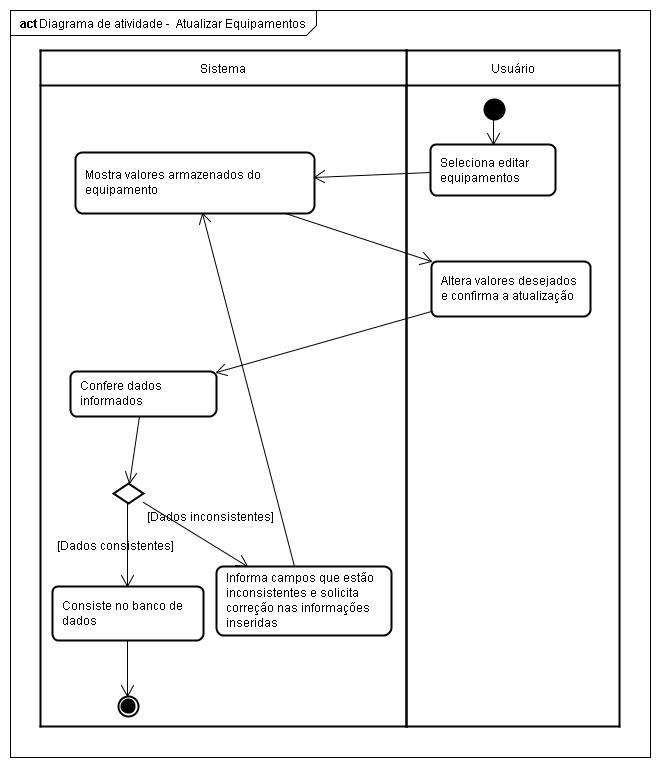
\includegraphics[width=14cm, height=15cm]{imagens-tc2/atividades/atualizarequipamentos.jpg}
%\caption{Diagrama de atividade - Atualizar Equipamentos}
\label{fig:Diagrama de atividade - Atualizar Equipamentos}
\end{figure}
\begin{figure}
\centering
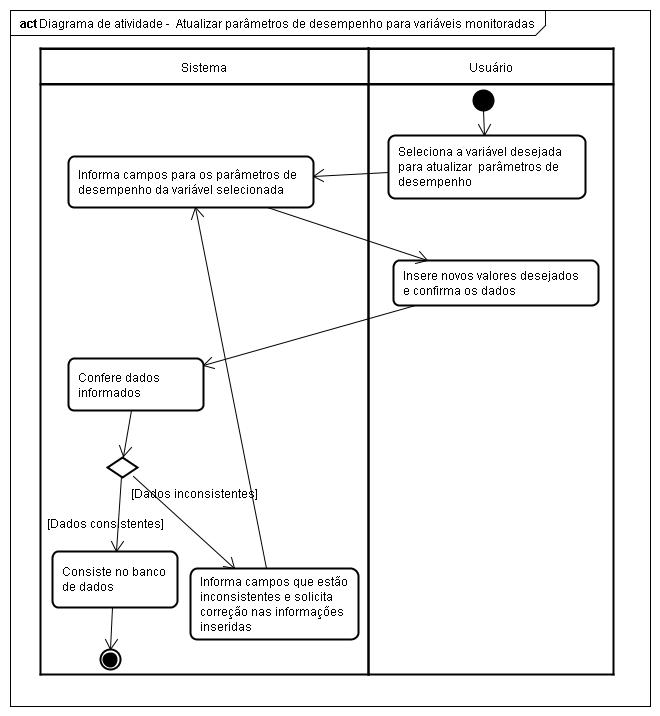
\includegraphics[width=15cm, height=20cm]{imagens-tc2/atividades/atualizarparametros.jpg}
%\caption{Diagrama de atividade - Atualizar par�metros de desempenho para vari�veis monitoradas}
\label{fig:Diagrama de atividade - Atualizar par�metros de desempenho para vari�veis monitoradas}
\end{figure}
\begin{figure}
\centering
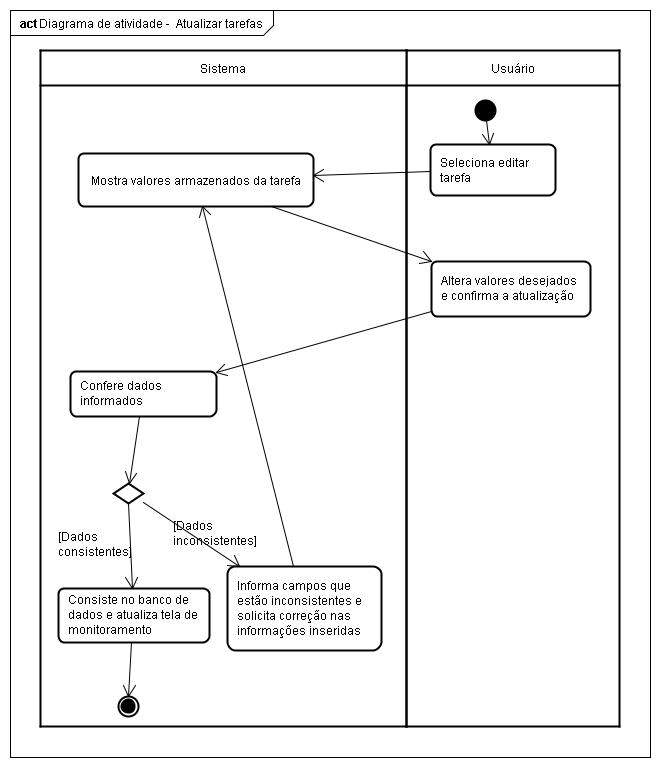
\includegraphics[width=15cm, height=20cm]{imagens-tc2/atividades/atualizartarefas.jpg}
%\caption{Diagrama de atividade - Atualizar tarefas}
\label{fig:Diagrama de atividade - Atualizar tarefas}
\end{figure}
\begin{figure}
\centering
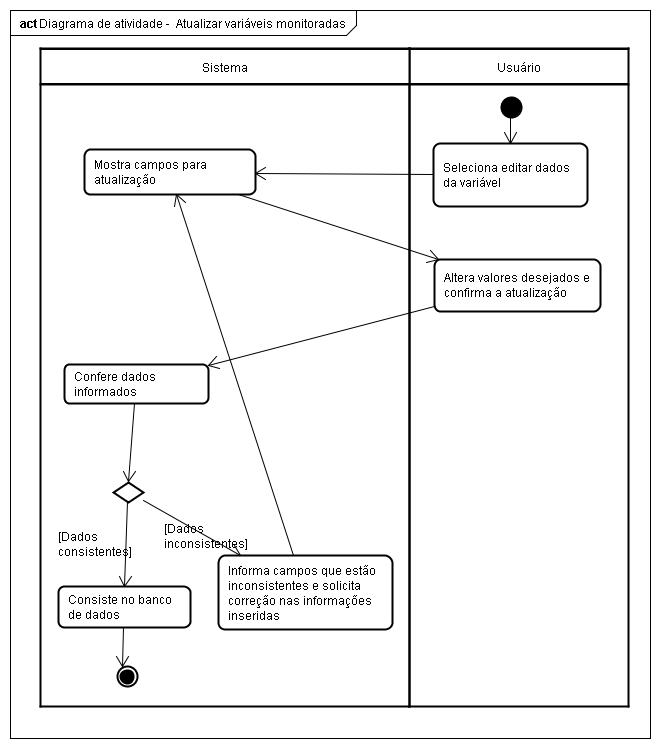
\includegraphics[width=15cm, height=20cm]{imagens-tc2/atividades/atualizarvariaveis.jpg}
%\caption{Diagrama de atividade - Atualizar vari�veis monitoradas}
\label{fig:Diagrama de atividade - Atualizar vari�veis monitoradas}
\end{figure}
\begin{figure}
\centering
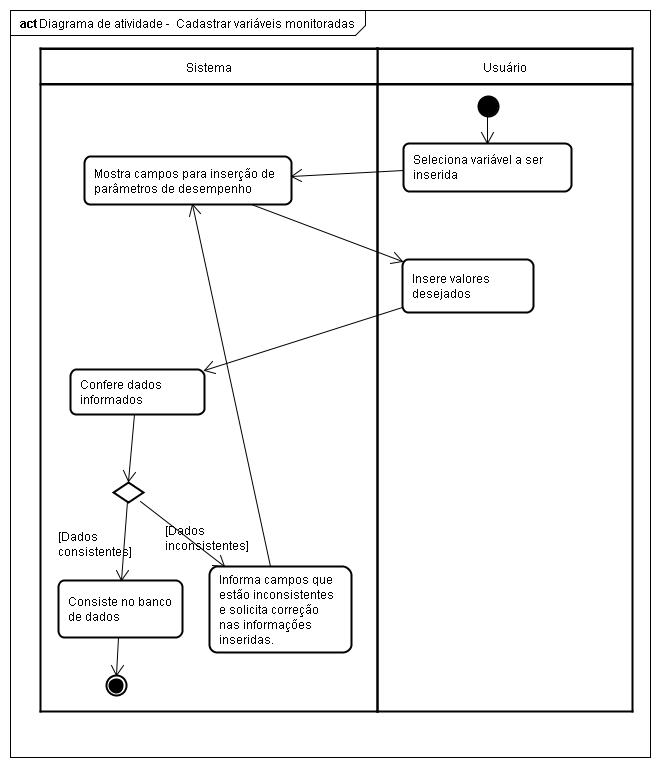
\includegraphics[width=15cm, height=20cm]{imagens-tc2/atividades/cadastrarvariaveis.jpg}
%\caption{Diagrama de atividade - Cadastrar vari�veis monitoradas}
\label{fig:Diagrama de atividade - Cadastrar vari�veis monitoradas}
\end{figure}
\begin{figure}
\centering
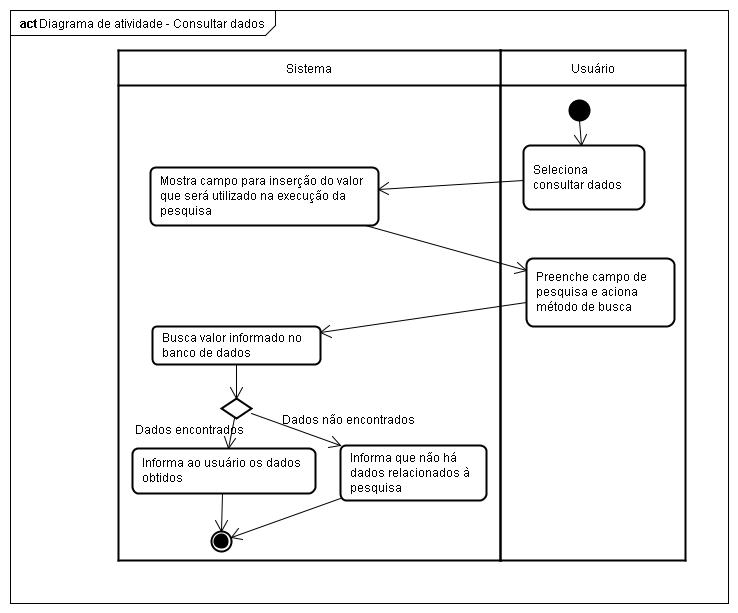
\includegraphics[width=15cm, height=20cm]{imagens-tc2/atividades/consultardados.jpg}
%\caption{Diagrama de atividade - Consultar dados}
\label{fig:Diagrama de atividade - Consultar dados}
\end{figure}
\begin{figure}
\centering
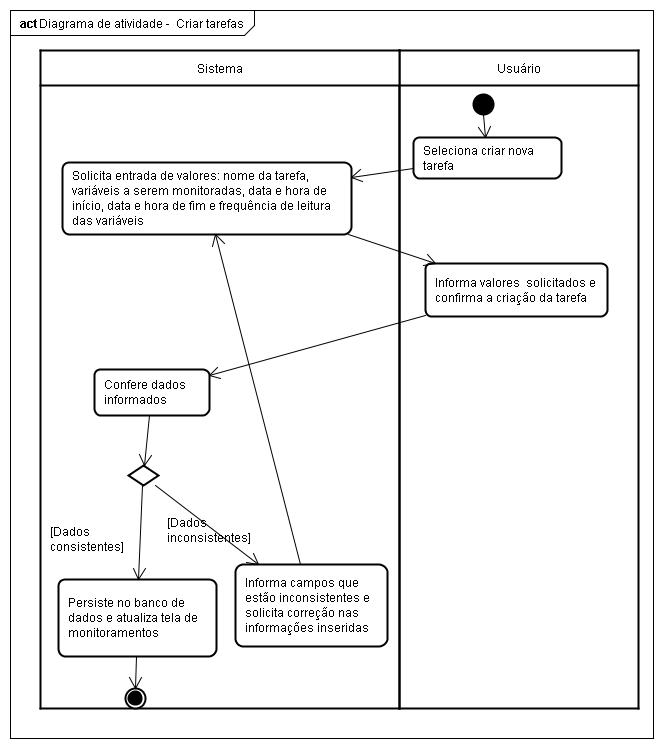
\includegraphics[width=15cm, height=20cm]{imagens-tc2/atividades/criartarefas.jpg}
%\caption{Diagrama de atividade - Criar tarefas}
\label{fig:Diagrama de atividade - Criar tarefas}
\end{figure}
\begin{figure}
\centering
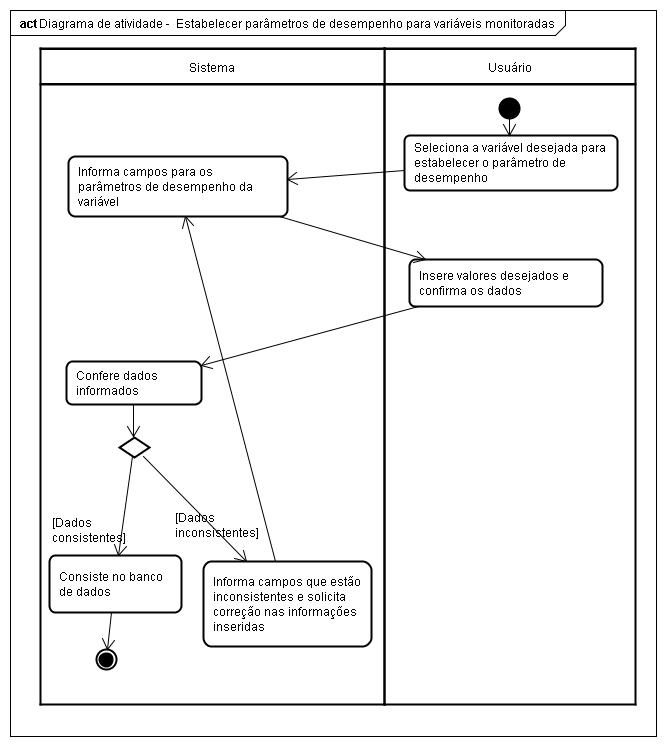
\includegraphics[width=15cm, height=20cm]{imagens-tc2/atividades/estabelecerparametros.jpg}
%\caption{Diagrama de atividade - Estabelecer par�metros de desempenho para vari�veis monitoradas}
\label{fig:Diagrama de atividade - Estabelecer par�metros de desempenho para vari�veis monitoradas}
\end{figure}
\begin{figure}
\centering
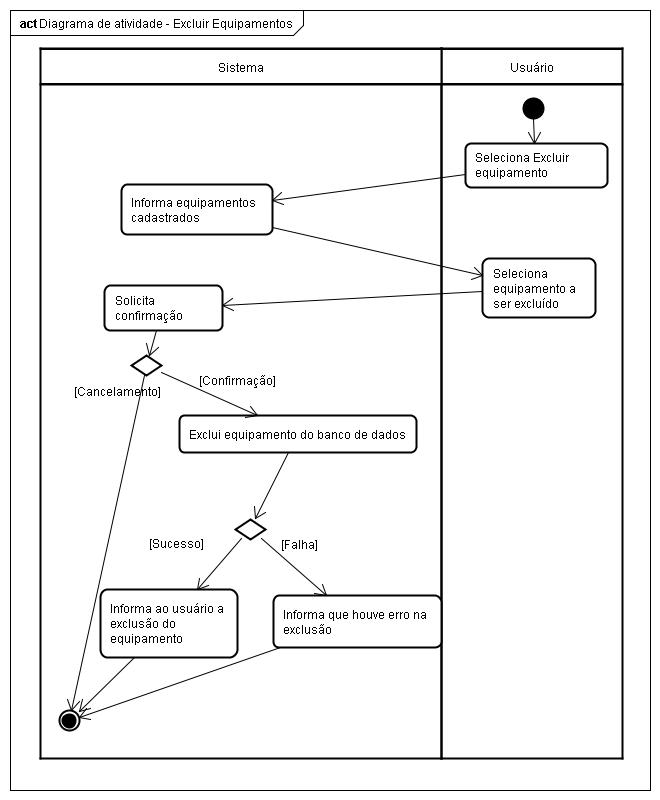
\includegraphics[width=15cm, height=20cm]{imagens-tc2/atividades/excluirequipamentos.jpg}
%\caption{Diagrama de atividade - Excluir Equipamentos}
\label{fig:Diagrama de atividade - Excluir Equipamentos}
\end{figure}
\begin{figure}
\centering
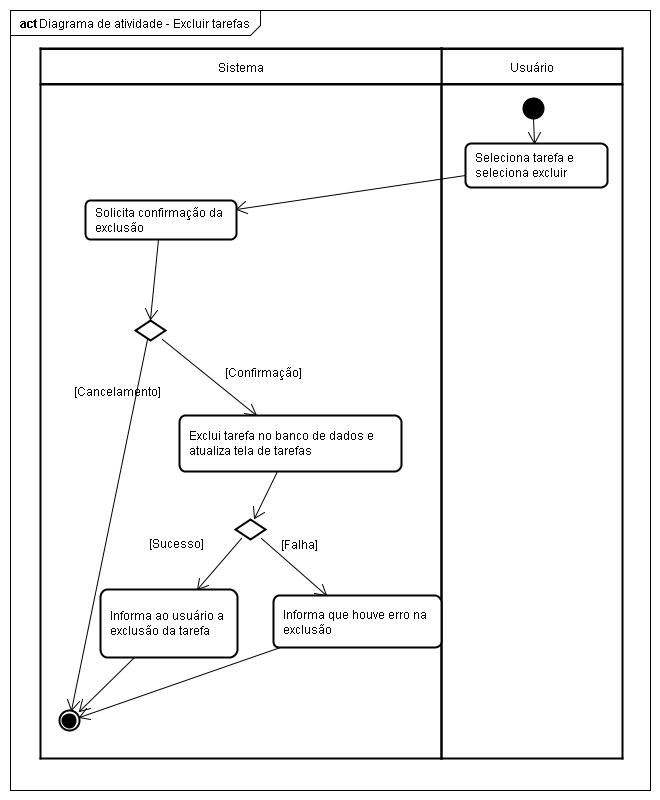
\includegraphics[width=15cm, height=20cm]{imagens-tc2/atividades/excluirtarefas.jpg}
%\caption{Diagrama de atividade - Excluir tarefas}
\label{fig:Diagrama de atividade - Excluir tarefas}
\end{figure}
\begin{figure}
\centering
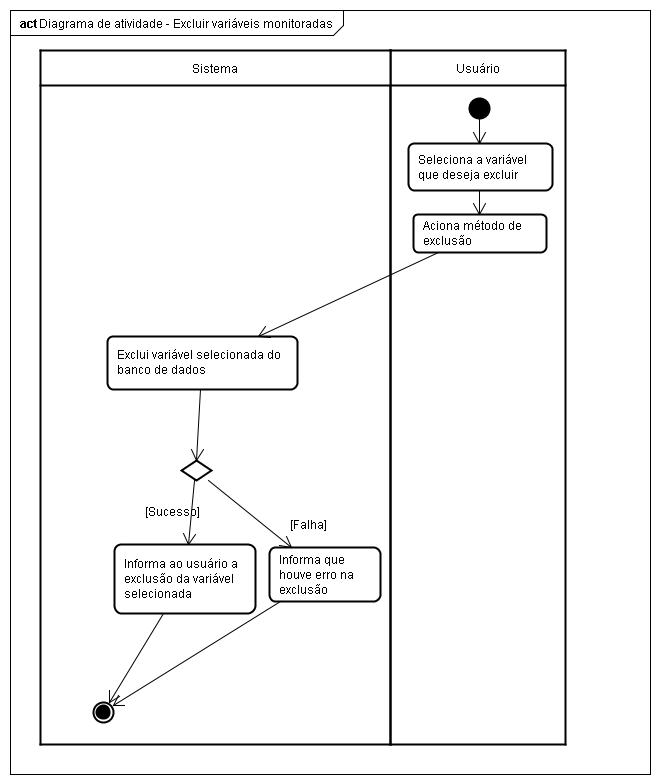
\includegraphics[width=15cm, height=20cm]{imagens-tc2/atividades/excluirvariaveis.jpg}
%\caption{Diagrama de atividade - Excluir vari�veis monitoradas}
\label{fig:Diagrama de atividade - Excluir vari�veis monitoradas}
\end{figure}
\begin{figure}
\centering
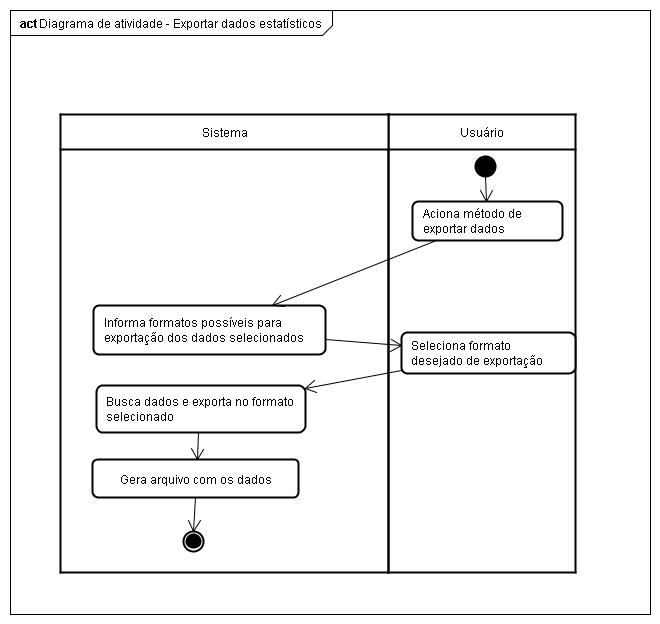
\includegraphics[width=15cm, height=20cm]{imagens-tc2/atividades/exportardados.jpg}
%\caption{Diagrama de atividade - Exportar dados estat�sticos}
\label{fig:Diagrama de atividade - Exportar dados estat�sticos}
\end{figure}
\begin{figure}
\centering
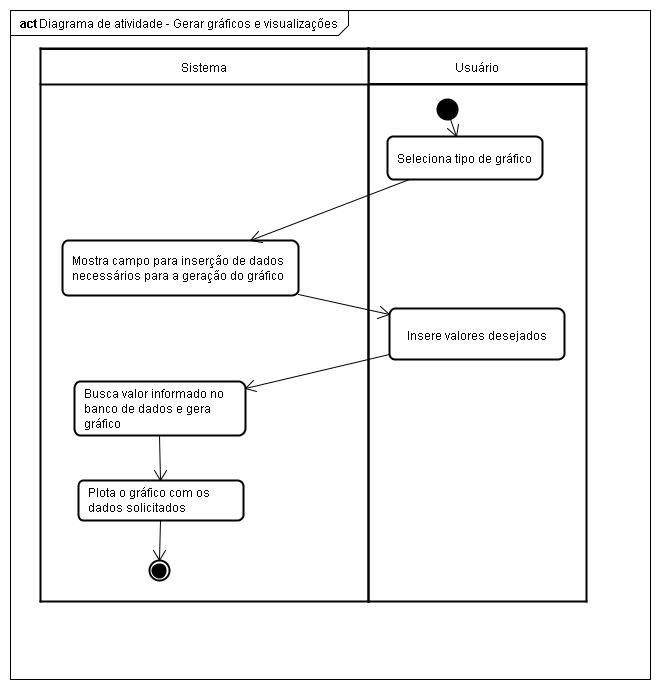
\includegraphics[width=15cm, height=20cm]{imagens-tc2/atividades/gerargraficos.jpg}
%\caption{Diagrama de atividade - Gerar gr�ficos e visualiza��es}
\label{fig:Diagrama de atividade - Gerar gr�ficos e visualiza��es}
\end{figure}
\begin{figure}
\centering
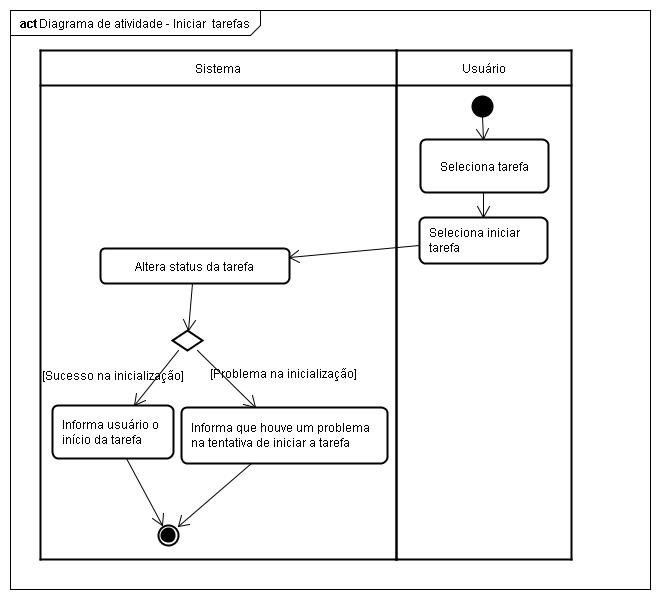
\includegraphics[width=15cm, height=20cm]{imagens-tc2/atividades/iniciartarefas.jpg}
%\caption{Diagrama de atividade - Iniciar tarefas}
\label{fig:Diagrama de atividade - Iniciar tarefas}
\end{figure}
\begin{figure}
\centering
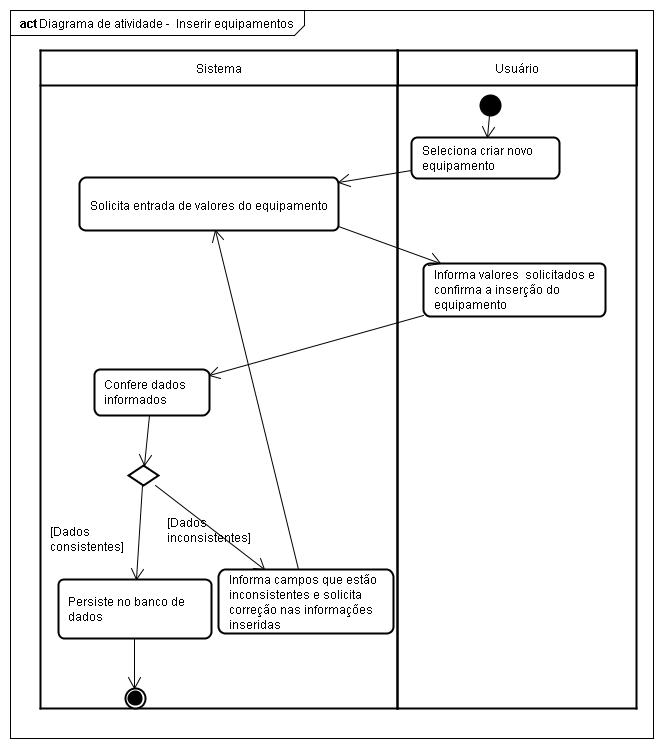
\includegraphics[width=15cm, height=20cm]{imagens-tc2/atividades/inserirequipamentos.jpg}
%\caption{Diagrama de atividade - Inserir equipamentos}
\label{fig:Diagrama de atividade - Inserir equipamentos}
\end{figure}
\begin{figure}
\centering
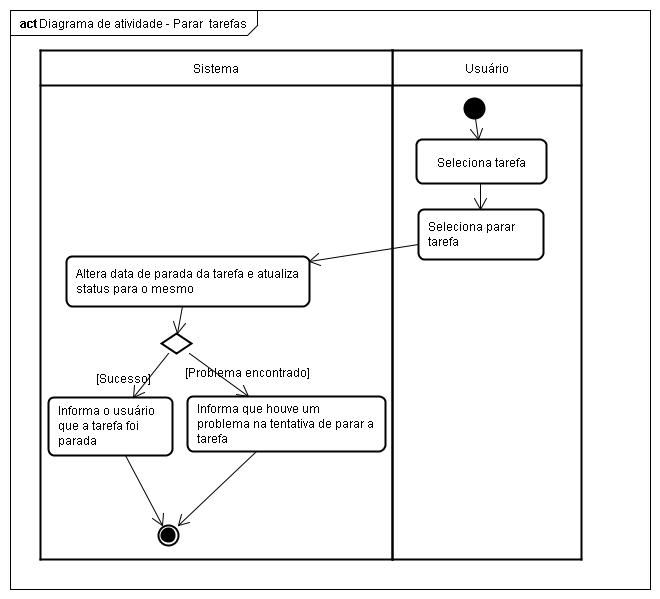
\includegraphics[width=15cm, height=20cm]{imagens-tc2/atividades/parartarefas.jpg}
%\caption{Diagrama de atividade - Parar tarefas}
\label{fig:Diagrama de atividade - Parar tarefas}
\end{figure}

\chapter*{Anexo B --- Diagramas de Classes}
\label{anexo}
%\addtocontents{toc}{\protect\contentsline {chapter}{Anexo B --- Diagramas de Classes}{74}}
Neste anexo s�o apresentados os diagramas de classes UML modelados para a implementa��o do sistema. S�o apresentados os diagrama de classes, inicialmente uma figura contendo todos os pacotes e classes (Figura \ref{classes:all}). A seguir cada um dos pacotes � melhor detalhado nas demais figuras.
\par O pacote \textit{model} cont�m as classes que s�o as entidades do programa, os DAOs de acesso �s entidades e enumera��es utilizadas nas classes entidades (Figura \ref{classes:model}).
\par O pacote \textit{controller} cont�m as classes de controle de acesso �s classes DAOs e classes de acesso ao protocolo SNMP (Figura \ref{classes:controller}).
\par O pacote \textit{util} cont�m as classes de utilidades do sistema, como configura��o de acesso ao banco de dados, exporta��o de dados, mensagens de erros do sistema, escalonador de leituras e classe inicial do sistema (Figura \ref{classes:util}).
\par Os pacotes \textit{graphics} e \textit{charts} cont�m as classes que geram as visualiza��es do sistema (Figura \ref{classes:graphics} e Figura \ref{classes:charts}).
\par E, o pacote \textit{view} cont�m as classes que representam as janelas e interfaces gr�ficas do sistema (Figura \ref{classes:view}).
\begin{figure}
\centering
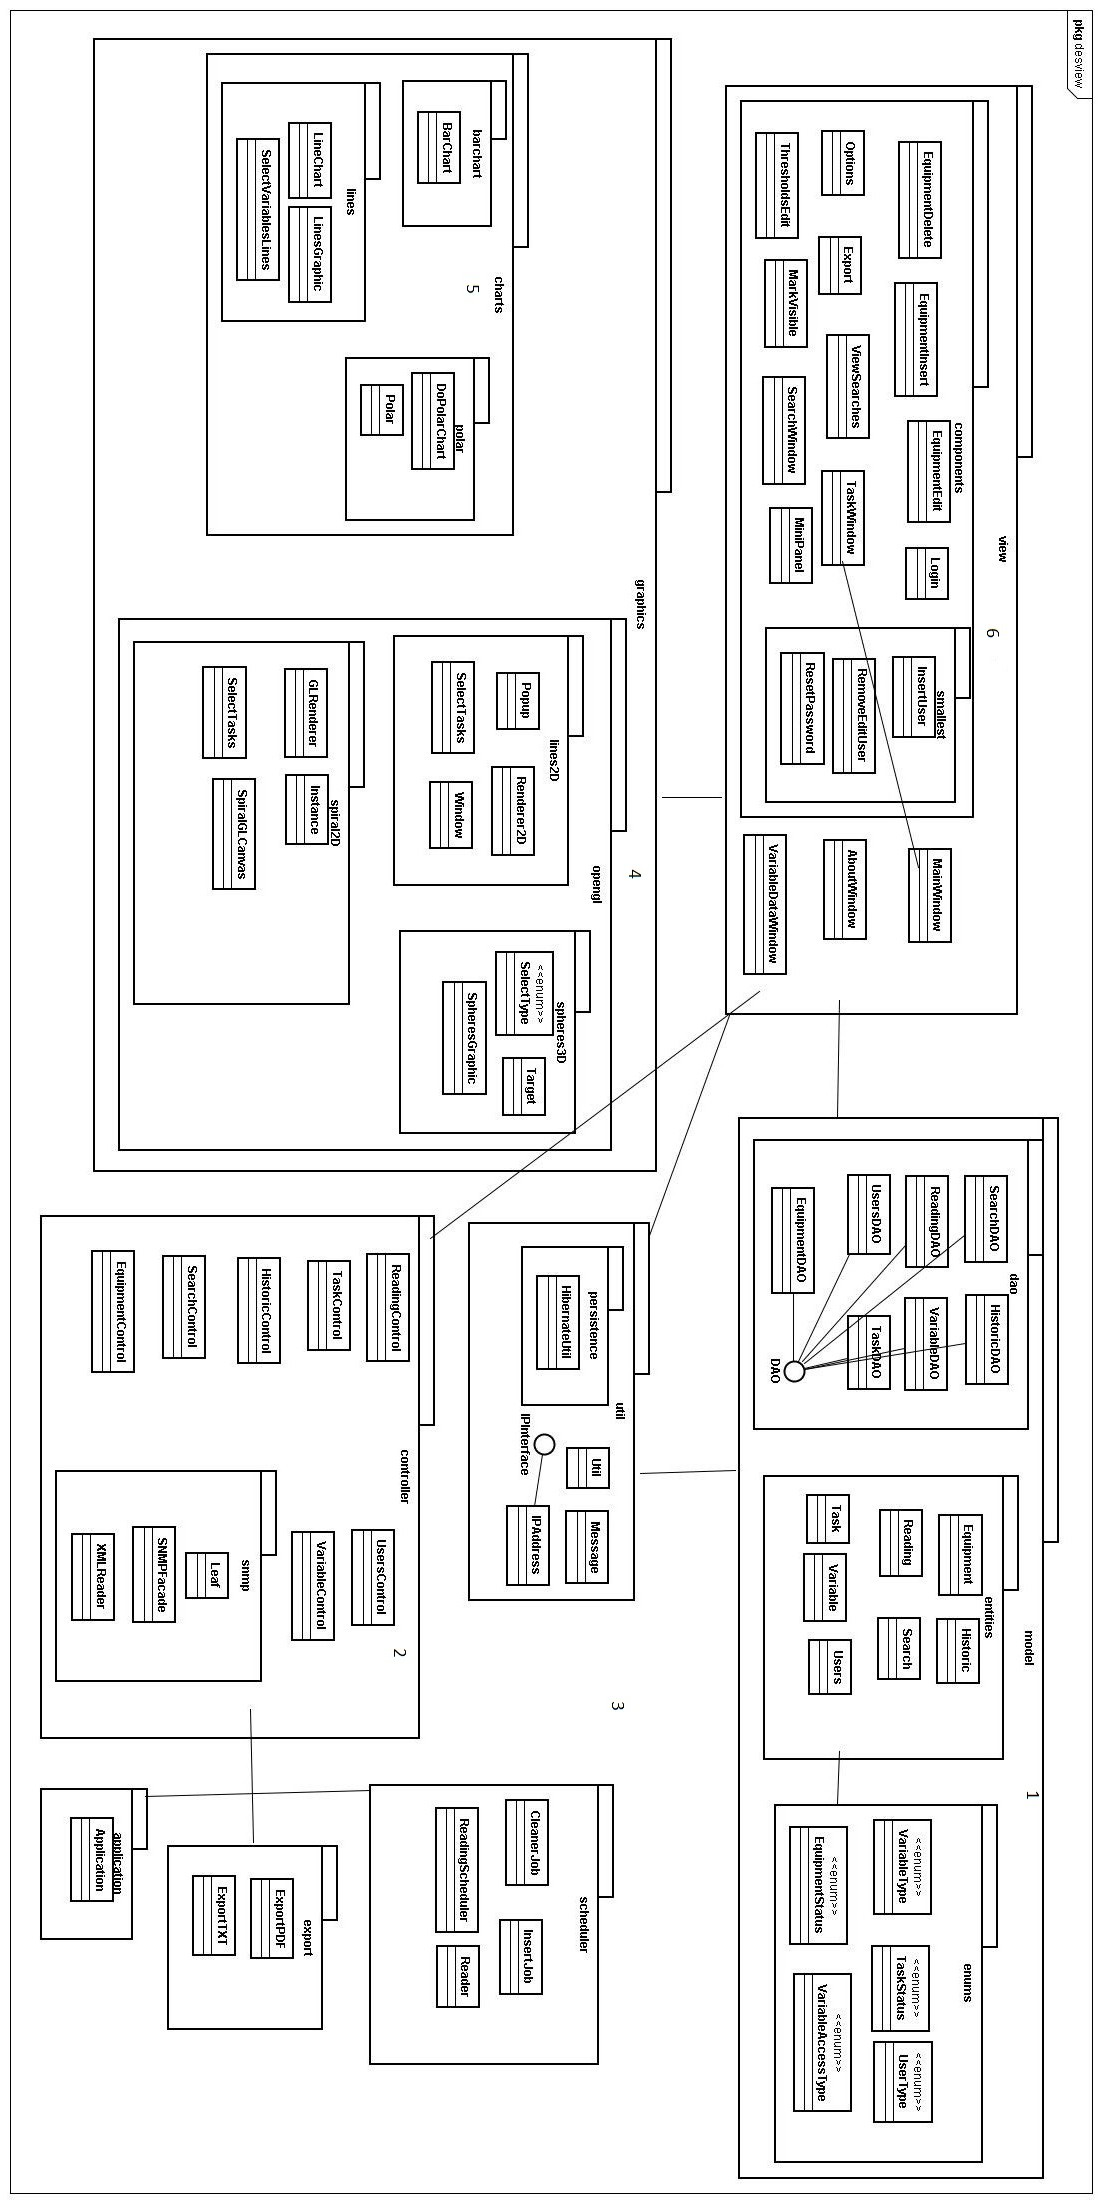
\includegraphics[width=16cm, height=20cm]{imagens-tc2/classes/allclasses.jpg}
\caption{Modelo conceitual de classes do sistema}
\label{classes:all}
\end{figure}
\begin{figure}
\centering
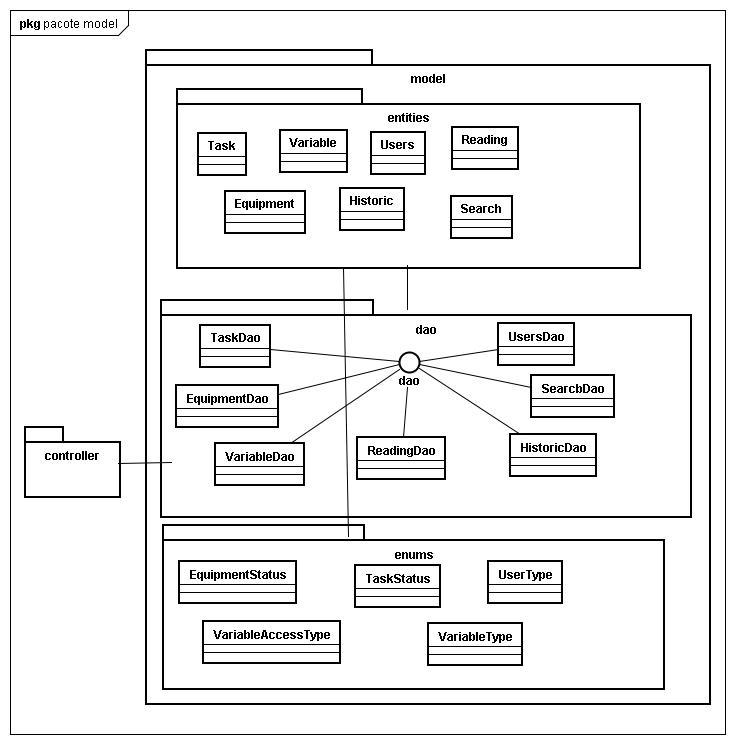
\includegraphics[width=15cm, height=20cm]{imagens-tc2/classes/model.jpg}
\caption{Modelo conceitual de classes: parte 1 - pacote \textit{model}.}
\label{classes:model}
\end{figure}
\begin{figure}
\centering
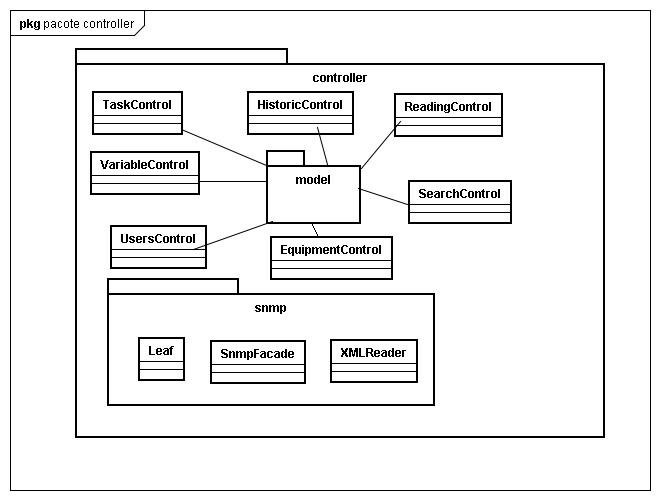
\includegraphics[width=15cm, height=20cm]{imagens-tc2/classes/controller.jpg}
\caption{Modelo conceitual de classes: parte 2 - pacote \textit{controller}.}
\label{classes:controller}
\end{figure}
\begin{figure}
\centering
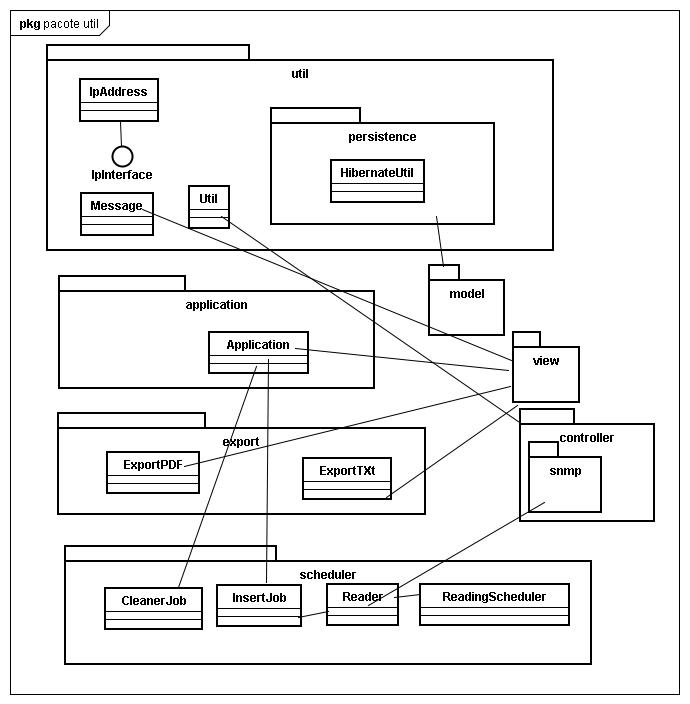
\includegraphics[width=15cm, height=20cm]{imagens-tc2/classes/util.jpg}
\caption{Modelo conceitual de classes: parte 3 - pacote \textit{util}.}
\label{classes:util}
\end{figure}
\begin{figure}
\centering
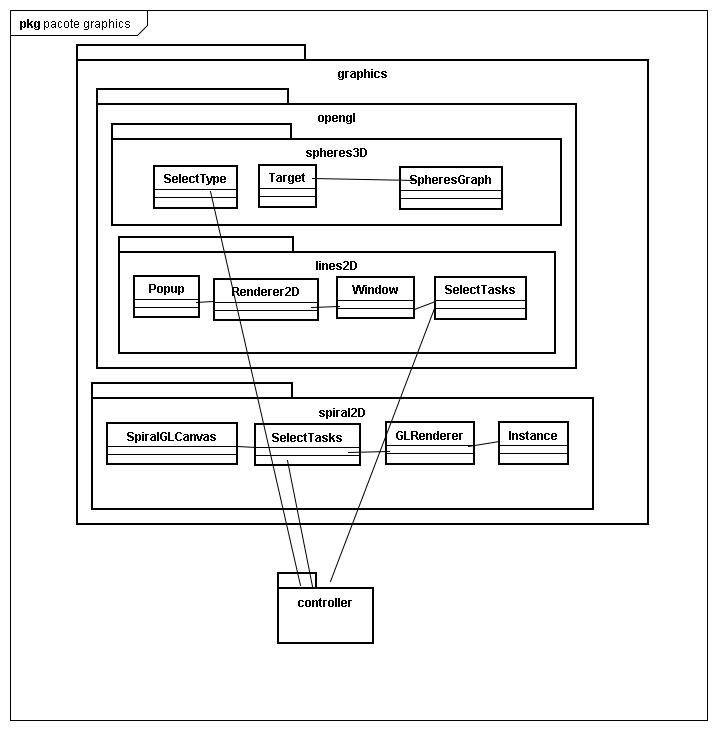
\includegraphics[width=15cm, height=20cm]{imagens-tc2/classes/graphics.jpg}
\caption{Modelo conceitual de classes: parte 4 - pacote \textit{graphics}.}
\label{classes:graphics}
\end{figure}
\begin{figure}
\centering
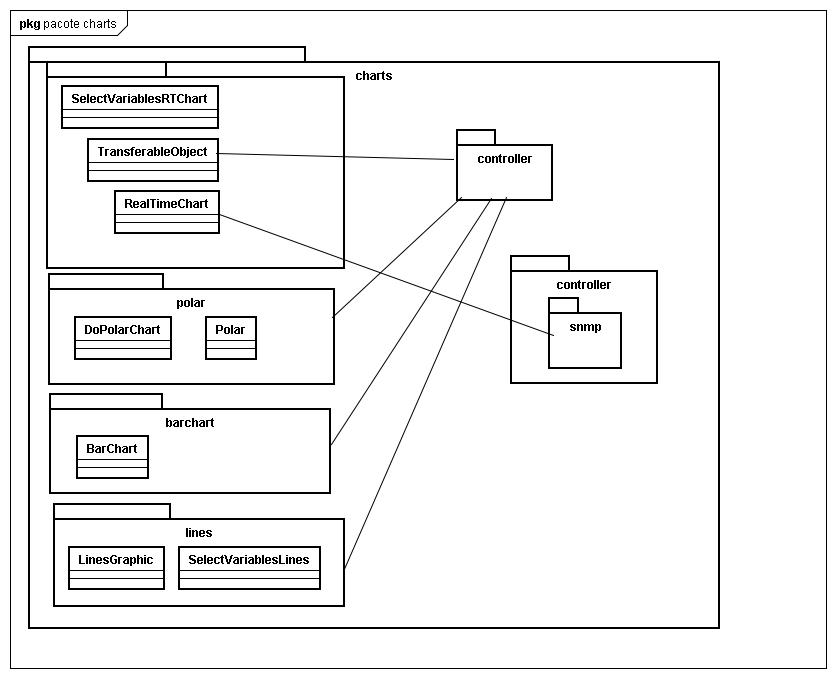
\includegraphics[width=15cm, height=20cm]{imagens-tc2/classes/charts.jpg}
\caption{Modelo conceitual de classes: parte 5 - pacote \textit{chart}s.}
\label{classes:charts}
\end{figure}
\begin{figure}
\centering
\includegraphics[width=15cm, height=20cm]{imagens-tc2/classes/view.jpg}
\caption{Modelo conceitual de classes: parte 6 - pacote \textit{view}.}
\label{classes:view}
\end{figure}


\chapter*{Anexo C --- Manual de utiliza��o}
\label{manual}
%\addtocontents{toc}{\protect\contentsline {chapter}{Anexo C --- Manual de utiliza��o}{82}}
Neste anexo � apresentado o manual de utiliza��o do sistema Desview. � mostrado como inserir equipamentos, tarefas e vari�veis no prot�tipo e como utilizar as visualiza��es implementadas.
\section*{\textit{Login}}
Para utilizar o sistema � necess�rio possuir uma conta com usu�rio e senha. Assim, a tela de \textit{login} � mostrada no in�cio da aplica��o, como ilustra a Figura \ref{fig:login}. Caso n�o possuir um usu�rio, crie um, e se esquecer da senha utilize o \textit{link} de recupera��o de senha.
\begin{figure}[!h]
\centering
\includegraphics[width=8cm, height=5cm]{imagens-tc2/manual/login.jpg}
\caption{Tela de \textit{login} do sistema.}
\label{fig:login}
\end{figure}
\section*{Inser��o de equipamentos, de tarefas e de vari�veis}
\label{sec:insere}
Ap�s entrar no sistema � aberta a tela inicial do sistema, conforme ilustra a Figura \ref{fig:telaprincipal}. Para iniciar as monitora��es � necess�rio inserir equipamentos e a seguir inserir tarefas, com vari�veis de MIB a serem monitoradas.
\par Para inserir equipamentos e tarefas, utilize o menu \textit{Tools}, a seguir selecione \textit{Insert} e \textit{Equipment} ou \textit{Task} (Figura \ref{fig:inserir-equip}). Tamb�m � poss�vel inserir tarefas atrav�s do bot�o \textit{New} da janela principal.
\begin{figure}
\centering
\includegraphics[width=12cm]{imagens-tc2/manual/telaprincipal.jpg}
\caption{Tela inicial do sistema com tarefas e visualiza��es.}
\label{fig:telaprincipal}
\end{figure}
\begin{figure}
\centering
\includegraphics[width=8cm, height=3cm]{imagens-tc2/manual/inserir-equip.jpg}
\caption{Inserindo equipamentos e tarefas.}
\label{fig:inserir-equip}
\end{figure}
\par Ao inserir equipamentos, � necess�rio informar o IP do equipamento, o nome do equipamento, comunidade de leitura e de escrita, \textit{timeout}, n�mero de \textit{retries} e porta de acesso SNMP, como apresentado na Figura \ref{fig:inserir-equip-dados}.
\par Para inserir tarefas, os dados necess�rios s�o os seguintes: nome da tarefa, equipamento em que ser� efetuada a leitura das vari�veis, vari�veis de MIB a serem monitoradas, data de in�cio e fim e intervalo entre as leituras, como apresentado na Figura \ref{fig:insere-task}. Cada vari�vel a ser inserida pode possuir \textit{thresholds} superior e inferior ao serem monitoradas. Para inserir os \textit{thresholds}, selecione um elemento da �rvore apresentada na Figura \ref{fig:insere-task}, � esquerda e selecione \textit{Insert \& Thresholds}. Ser� apresentada a janela de edi��o dos valores ilustrada na Figura \ref{fig:thresholds}, na qual deve ser inseridos e salvos os valores desejados. A vari�vel � ent�o adicionada � tarefa e passa a ser monitorada juntamente com as demais vari�veis que venham a ser adicionadas � tarefa.
\begin{figure}
\centering
\includegraphics[width=8cm, height=5cm]{imagens-tc2/manual/inserir-equipamento.jpg}
\caption{Inser��o de equipamentos.}
\label{fig:inserir-equip-dados}
\end{figure}
\begin{figure}
\centering
\includegraphics[width=8cm, height=7cm]{imagens-tc2/manual/inserirtarefa.jpg}
\caption{Inser��o de tarefas e vari�veis.}
\label{fig:insere-task}
\end{figure}
\begin{figure}
\centering
\includegraphics[width=8cm, height=3cm]{imagens-tc2/manual/thresholds.jpg}
\caption{Defini��o de \textit{thresholds} de vari�veis.}
\label{fig:thresholds}
\end{figure}
\section*{Edi��o de equipamentos, de tarefas e de vari�veis}
Para editar um equipamento, uma tarefa ou dados de uma vari�vel associada a uma tarefa deve-se utilizar o menu \textit{Tools}, \textit{Edit} e a seguir \textit{Equipment} ou \textit{Task}, como representado na Figura \ref{fig:editar}. Nas janelas de edi��o dos dados j� cadastrados que ser�o apresentadas, deve-se inserir e salvar as altera��es desejadas.
\begin{figure}[!h]
\centering
\includegraphics[width=8cm, height=3cm]{imagens-tc2/manual/editar.jpg}
\caption{Edi��o de equipamentos e tarefas.}
\label{fig:editar}
\end{figure}
\section*{Remo��o de equipamentos, tarefas e vari�veis}
Para remover uma tarefa selecione a tarefa desejada na tabela de tarefas em monitora��o da janela principal (Figura \ref{fig:telaprincipal}), utilize o menu \textit{Tools}, \textit{Delete} e a seguir \textit{Task}, como representado na Figura \ref{fig:remover}. Para remover um equipamento inicialmente selecione \textit{Equipment}, ap�s ser� apresentada uma janela como a mostrada na Figura \ref{fig:removerequipamento}, escolha o equipamento desejado e remova-o. Tamb�m � poss�vel tornar uma tarefa invis�vel, ou seja, apenas mantendo-a no banco de dados, por�m sem aparecer na janela de tarefas e sem efetuar leituras. Assim, os dados estat�sticos da mesma n�o s�o removidos do banco de dados. Para remover vari�veis abra a tarefa desejada e remova utilizando o bot�o \textit{Remove}, mostrado na Figura \ref{fig:insere-task}.
\begin{figure}
\centering
\includegraphics[width=8cm, height=3cm]{imagens-tc2/manual/remover.jpg}
\caption{Remover de equipamentos e tarefas.}
\label{fig:remover}
\end{figure}
\begin{figure}
\centering
\includegraphics[width=10cm, height=5cm]{imagens-tc2/manual/removerequipamento.jpg}
\caption{Janela de escolha de equipamento a ser deletado.}
\label{fig:removerequipamento}
\end{figure}
\section*{Parar e iniciar tarefas}
As tarefas cadastradas que estejam executando podem ser paradas caso desejado. Tamb�m � poss�vel iniciar uma tarefa que esteja parada. Essas a��es podem ser executadas atrav�s dos bot�es \textit{Start} e \textit{Stop}, mostrados na Figura \ref{fig:botoes}. Tarefas que possuem o estado \textit{Stopped} n�o s�o lidas pelo escalonador, ou seja, n�o realizam consultas SNMP nem inserem o resultado das consultas no banco de dados. Tamb�m � poss�vel atualizar a tela com as tarefas e verificar o estado de cada uma das tarefas, criar uma nova tarefa e editar uma tarefa j� cadastrada. 
\begin{figure}[!h]
\centering
\includegraphics[width=7cm, height=2cm]{imagens-tc2/manual/botoes.jpg}
\caption{Bot�es de a��es para as tarefas.}
\label{fig:botoes}
\end{figure}
\section*{Exportar dados}
O prot�tipo permite exportar dados nos formatos texto (TXT) e PDF. Para exportar os dados lidos de leituras, deve-se utilizar o menu \textit{File}, a seguir \textit{Export}. Escolha o formato de exporta��o como mostrado na Figura \ref{fig:export}. A seguir, informe o diret�rio a ser salvo o arquivo.
\begin{figure}[!h]
\centering
\includegraphics[width=7cm, height=4cm]{imagens-tc2/manual/telaexport.jpg}
\caption{Tela de escolha de formatos de exporta��o.}
\label{fig:export}
\end{figure}
\section*{Utilizando as visualiza��es}
S�o oferecidas as seguintes visualiza��es no sistema (Figura \ref{fig:visualizations}):
\begin{itemize}
\item Visualiza��o em linhas;
\item Visualiza��o em espirais;
\item Visualiza��o em esferas;
\item \textit{Chart} de monitora��o em tempo real de vari�veis;
\item \textit{Chart} polar, de barras e de linhas.
\end{itemize}
\begin{figure}[!h]
\centering
\includegraphics[width=7cm]{imagens-tc2/manual/visulizations.jpg}
\caption{Tela de escolha de visualiza��es a serem plotadas.}
\label{fig:visualizations}
\end{figure}
\subsection*{Visualiza��es em \textit{charts}}
O \textit{chart} de tempo real tem por objetivo a monitora��o de at� 5 vari�veis de diferentes tarefas e assim, verificar o valor atual de cada uma vari�veis e monitor�-las a partir de um \textit{threshold}, informando se algum dos valores lidos das vari�veis passou do \textit{threshold} informado.
\begin{figure}[!h]
\centering
\includegraphics[width=7cm, height=5cm]{imagens-tc2/manual/escolhavariaveisrt.jpg}
\caption{Janela de escolha de vari�veis.}
\label{fig:escrt}
\end{figure}
\begin{figure}[!h]
\centering
\includegraphics[width=10cm, height=8cm]{imagens-tc2/manual/rt.jpg}
\caption{Exemplo de gr�fico de tempo real gerado.}
\label{fig:rt}
\end{figure}
\par Os demais \textit{charts} s�o utilizados para verificar estat�sticas das leituras efetuadas. O prot�tipo possui \textit{charts} em formato de barras, de linhas e gr�fico polar. Para utilizar informe os dados solicitados para constru��o do \textit{chart}, como: ano, m�s e vari�vel para que o gr�fico seja plotado.
\subsection*{Visualiza��es em OpenGL}
\subsubsection*{Gr�fico 2D de linhas e de espirais}
Para gerar os gr�ficos 2D de linhas ou de espirais, inicialmente � necess�rio escolher qual � a tarefa que se deseja visualizar, como mostrado na Figura \ref{fig:selecttask}, ap�s s�o gerados os gr�ficos mostrando se os valores lidos est�o dentro, acima ou abaixo do intervalo determinado como normal para a vari�vel, como mostrado na Figura \ref{fig:linhasespirais}, que apresenta os dois gr�ficos monitorando diferentes vari�veis.
\begin{figure}[!h]
\centering
\includegraphics[width=10cm, height=5cm]{imagens-tc2/manual/selecaotasklinhaseespirais.jpg}
\caption{Janela de sele��o de tarefas para gr�ficos OpenGL.}
\label{fig:selecttask}
\end{figure}
\begin{figure}[!h]
\centering
\includegraphics[width=10cm, height=5cm]{imagens-tc2/manual/linhas-espirais.jpg}
\caption{Exemplo de gr�fico de linhas e de espirais gerados.}
\label{fig:linhasespirais}
\end{figure}
\subsubsection*{Gr�fico 3D}
Para gerar os gr�ficos 3D de esferas, inicialmente � necess�rio escolher qual � a tarefa que se deseja visualizar, como mostrado na Figura \ref{fig:selecttask}. Ap�s s�o plotadas sequ�ncias de gr�ficos 3D informando as m�dias das vari�veis nos meses do ano e o estado da m�dia em rela��o aos \textit{thresholds}, ao clicar em uma das vari�veis � trazido a m�dia dos dias do ano Figura \ref{fig:3dm3}, novamente informando a m�dia em rela��o aos \textit{thresholds}. Dois exemplos de imagens geradas pela visualiza��o em esferas s�o mostrado na Figura \ref{fig:3dm} e Figura \ref{fig:3dm2}.
\begin{figure}
\centering
\includegraphics[width=10cm]{imagens-tc2/estudo-caso/3d1.jpg}
\caption{Exemplo 1 de gr�fico em esferas.}
\label{fig:3dm}
\end{figure}
\begin{figure}
\centering
\includegraphics[width=10cm]{imagens-tc2/estudo-caso/3d2.jpg}
\caption{Exemplo 2 de gr�fico em esferas.}
\label{fig:3dm2}
\end{figure}
\begin{figure}
\centering
\includegraphics[width=10cm]{imagens-tc2/revisao/3d2.png}
\caption{N�vel de dias de uma tarefa selecionada.}
\label{fig:3dm3}
\end{figure}


\end{document}
